%\chapter{Risultati numerici}
\section{Risultati numerici}
\label{chap:Results}
In questo capitolo verranno esposti i risultati numerici ottenuti.
I primi due esampi sono stati presi da \cite{MAIN}.
In entrambi questi esempi verrà considerato l'operatore lineare affine $\tilde{B}$ \ref{eq:210}.

\subsection{Test Case 01}
\subsubsection{Set-up}
Il primo esempio considerato, in accordo con l'ipotesi i) introdotta in Chapter \ref{chap:Continuo}.
Preso il dominio spazio-temporale $\Omega \times I = (0,1)^2 x(0,0.01)$ e d=1, si considera l'operatore di controllo lineare affine $\tilde{B}$ che può essere completamente caratterizato da:
{\renewcommand\arraystretch{2}
\begin{equation}
\begin{array}{c}
g_1(t,x_1,x_2) = sin({\pi}x_1)sin({\pi}x_2)\\
g_0(t,x_1,x_2) = -{\pi}^2w_a(t,x_1,x_2) - BP_{U_{ad}} \left( -\frac{1}{4\alpha}(exp(a{\pi}^2t)-exp(a{\pi}^2T)) \right)
\end{array}
\label{eq:500}
\end{equation}
}
dove
\begin{equation}
w_a(t,x_1,x_2) = exp(a{\pi}^2t)sin({\pi}x_1)sin({\pi}x_2) \text{, } a \in \mathbb{R}
\label{eq:501}
\end{equation}
In particolare vengono considerate le costanti $a=-\sqrt{5}$ ed $\alpha={pi}^{-4}$.
Come conseguenza di ciò si ha che \ref{eq:212} verrà riscritta, utilizzando l'aggiunto di B e non $\tilde{B}$, come:
\begin{equation}
(B'z)(t) = \int_{\Omega} z(t,x_1,x_2)g_1(t,x_1,x_2) ,dx_1dx_2
\label{eq:502}
\end{equation}
Si definiscono ora:
{\renewcommand\arraystretch{2}
\begin{equation}
\begin{array}{c}
y_d(t,x_1,x_2) = \frac{a^2 - 5}{2 + a}{pi}^2w_a(t,x_1,x_2) + 2{pi}^2w_a(T,x_1,x_2) \\
y_0(x_1,x_2) = \frac{- 1}{2 + a}{pi}^2w_a(0,x_1,x_2)
\end{array}
\label{eq:503}
\end{equation}
}
L'insieme ammissibile $U_{ad}$ è limitato inferiormente da $a_1=-25$ e superiormente da $b_1=-1$.
Infine definiamo le soluzioni esatte per il problema di controllo ottimo \ref{eq:200}:
{\renewcommand\arraystretch{2}
\begin{equation}
\begin{array}{c}
\overline{u}(t,x_1,x_2) = P_{U_{ad}} \left( -\frac{1}{4\alpha}(exp(a{\pi}^2t)-exp(a{\pi}^2T)) \right) \\
\overline{y}(t,x_1,x_2) = \frac{- 1}{2 + a}{pi}^2w_a(0,x_1,x_2) \\
\overline{p}(t,x_1,x_2) = w_a(t,x_1,x_2) - w_a(T,x_1,x_2)
\end{array}
\label{eq:504}
\end{equation}
}

\subsubsection{Risultati Numerici}
\begin{figure}
\centering
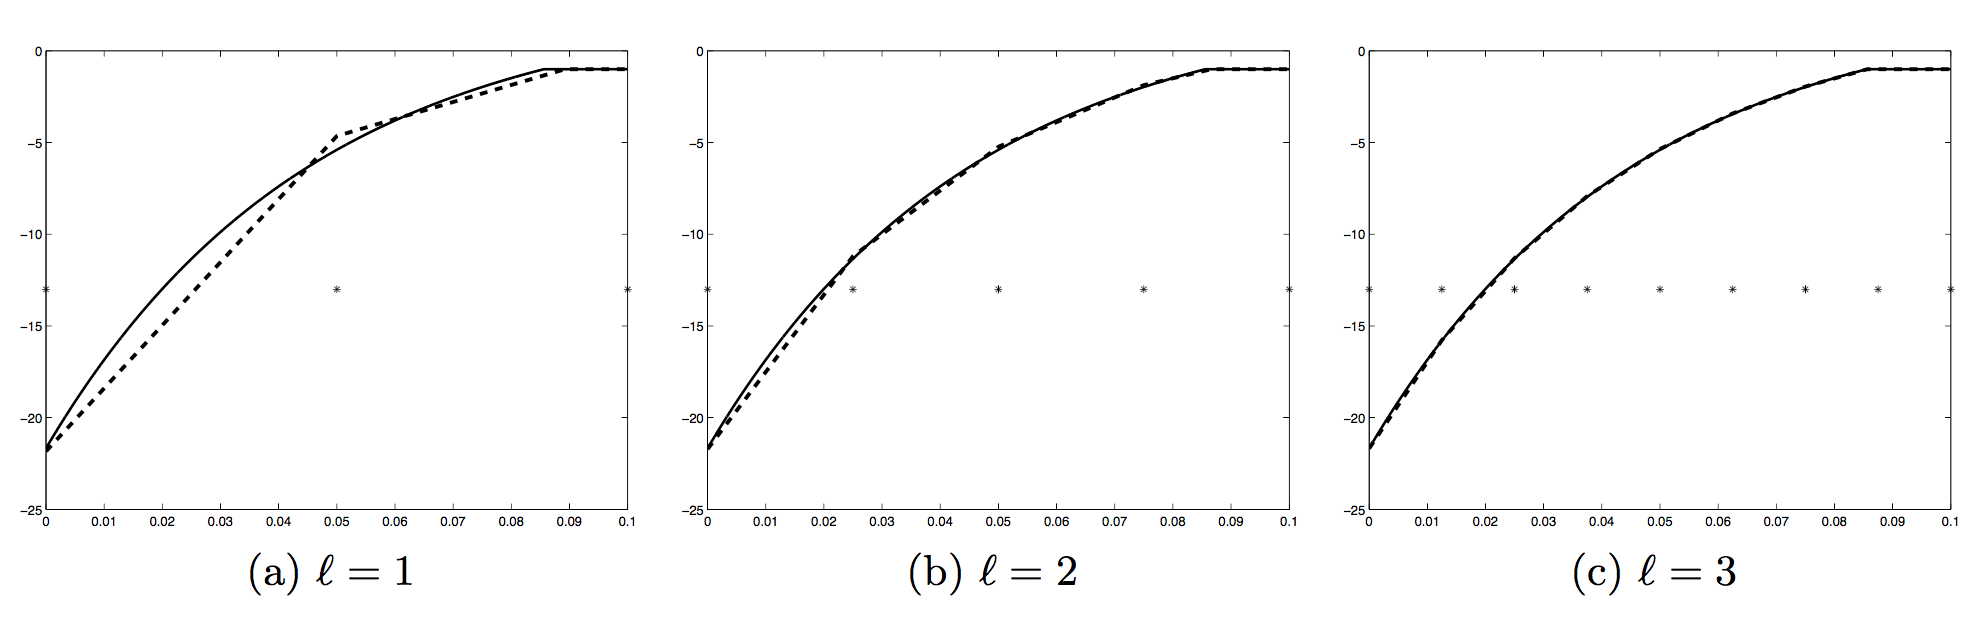
\includegraphics[width=\linewidth]{img/cap6/TestCase01_ues_paper}
\caption{Test Case 01 $\overline{u}$ e $u_k$ risultati di \cite{MAIN}}
\label{fig:500}
\end{figure}

\begin{figure}
\centering%
\subfigure[\protect\url{l = 1}]%
{\includegraphics[width=0.3\linewidth]{img/cap6/Imm_PF_01/ControlSol_N150_l1}}\qquad
\subfigure[\protect\url{l = 2}]%
{\includegraphics[width=0.3\linewidth]{img/cap6/Imm_PF_01/ControlSol_N150_l2}}\qquad
\subfigure[\protect\url{l = 3}]%
{\includegraphics[width=0.3\linewidth]{img/cap6/Imm_PF_01/ControlSol_N150_l3}}\qquad
\subfigure[\protect\url{l = 4}]%
{\includegraphics[width=0.3\linewidth]{img/cap6/Imm_PF_01/ControlSol_N150_l4}}\qquad
\subfigure[\protect\url{l = 5}]%
{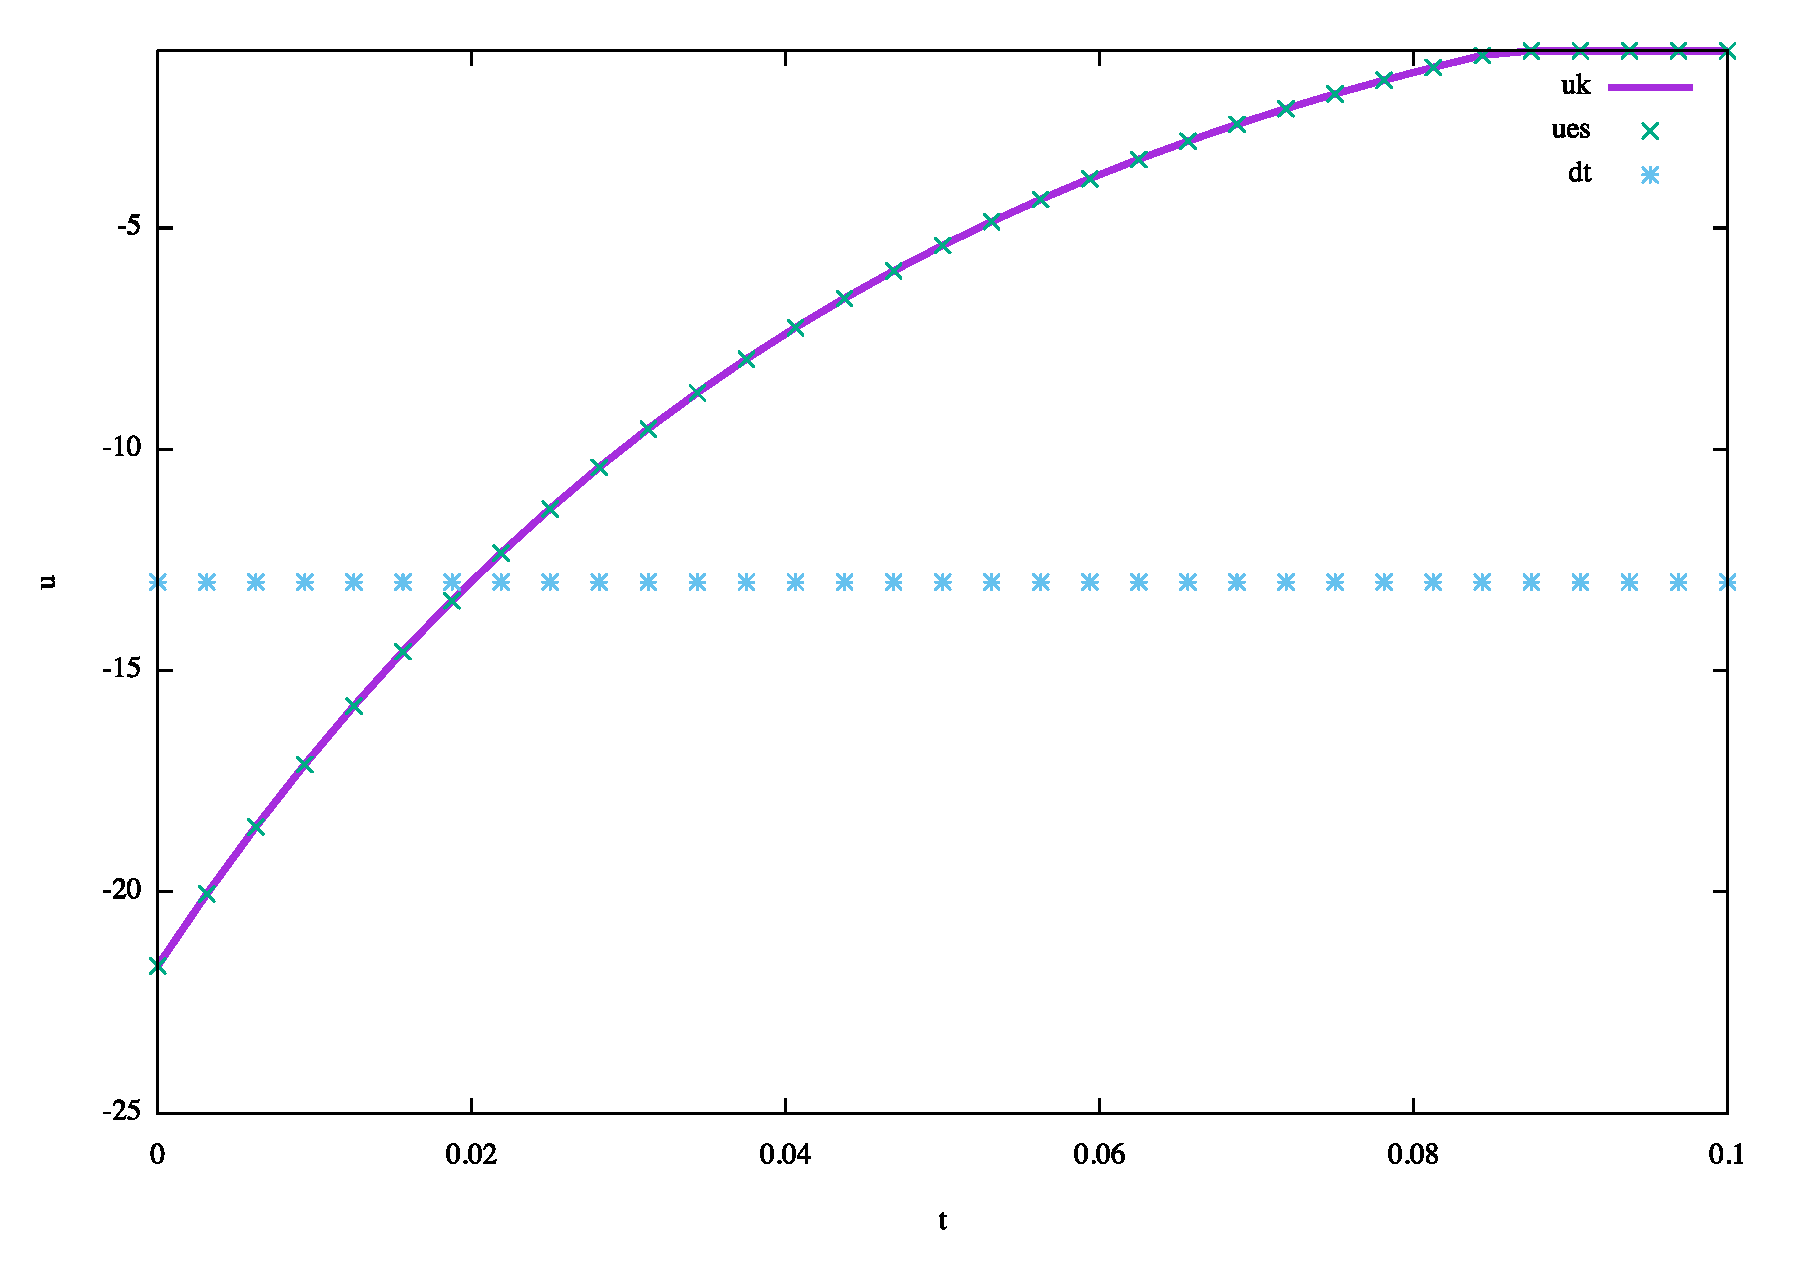
\includegraphics[width=0.3\linewidth]{img/cap6/Imm_PF_01/ControlSol_N150_l5}}\qquad
\subfigure[\protect\url{l = 6}]%
{\includegraphics[width=0.3\linewidth]{img/cap6/Imm_PF_01/ControlSol_N150_l6}}
\caption{Test Case 01 $\overline{u}$ e $u_k$ risultati dell'algoritmo di punto fisso}
\label{fig:501}
\end{figure}

\begin{figure}
\centering%
\subfigure[\protect\url{l = 1}]%
{\includegraphics[width=0.3\linewidth]{img/cap6/Imm_CG_01/ControlSol_N150_l1}}\qquad
\subfigure[\protect\url{l = 2}]%
{\includegraphics[width=0.3\linewidth]{img/cap6/Imm_CG_01/ControlSol_N150_l2}}\qquad
\subfigure[\protect\url{l = 3}]%
{\includegraphics[width=0.3\linewidth]{img/cap6/Imm_CG_01/ControlSol_N150_l3}}\qquad
\subfigure[\protect\url{l = 4}]%
{\includegraphics[width=0.3\linewidth]{img/cap6/Imm_CG_01/ControlSol_N150_l4}}\qquad
\subfigure[\protect\url{l = 5}]%
{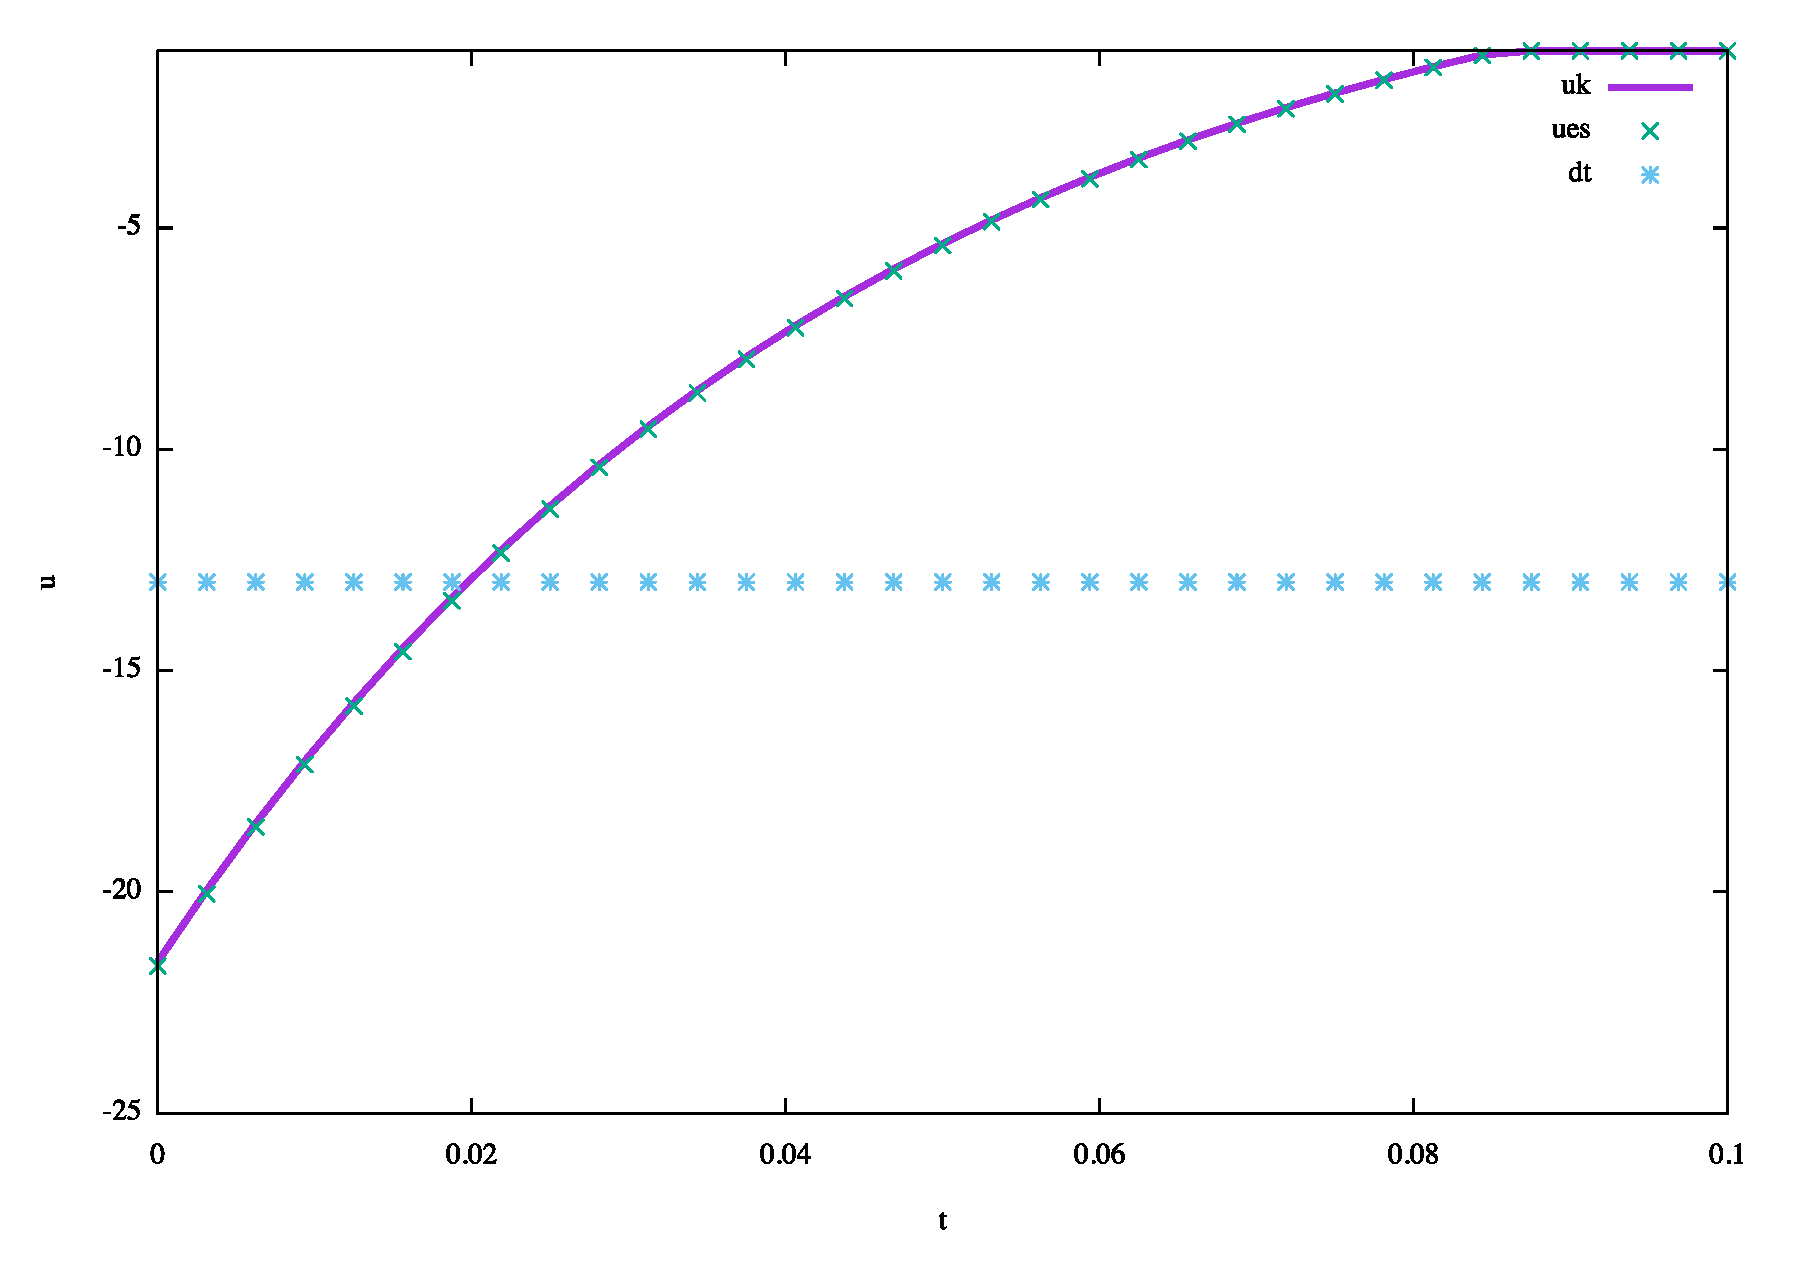
\includegraphics[width=0.3\linewidth]{img/cap6/Imm_CG_01/ControlSol_N150_l5}}\qquad
\subfigure[\protect\url{l = 6}]%
{\includegraphics[width=0.3\linewidth]{img/cap6/Imm_CG_01/ControlSol_N150_l6}}
\caption{Test Case 01 $\overline{u}$ e $u_k$: risultati dell'algortimod di semi newton}
\label{fig:502}
\end{figure}

\section{Test Case 02}
\subsubsection{Set-up}
Il primo esempio considerato, in accordo con l'ipotesi i) introdotta in Chapter \ref{chap:Continuo}.
Preso il dominio spazio-temporale $\Omega \times I = (0,1)^2 x(0,0.5)$ e d=1, si considera l'operatore di controllo lineare affine $\tilde{B}$ che può essere completamente caratterizato da:
{\renewcommand\arraystretch{2}
\begin{equation}
\begin{array}{c}
g_1(t,x_1,x_2) = sin({\pi}x_1)sin({\pi}x_2)\\
g_0(t,x_1,x_2) = g_1(t,x_1,x_2) 2\pi \left( -\frac{a}{T}sin\left( \frac{t}{T}2{\pi}a \right) + \pi cos\left( \frac{t}{T}2{\pi}a \right) \right) - B\overline{u}
\end{array}
\label{eq:505}
\end{equation}
}
In particolare vengono considerate le costanti $a=-2$ ed $\alpha=1$.
Si definiscono ora:
{\renewcommand\arraystretch{2}
\begin{equation}
\begin{array}{c}
y_d(t,x_1,x_2) = g_1\left( cos\left( \frac{t}{T}2{\pi}a \right)(1-2{\pi}^2) -\frac{2{\pi}a}{T}sin\left( \frac{t}{T}2{\pi}a \right) +2{\pi}^2cos(2{\pi}a) \right)\\
y_0(x_1,x_2) = g_1(t,x_1,x_2)
\end{array}
\label{eq:506}
\end{equation}
}
L'insieme ammissibile $U_{ad}$ è limitato inferiormente da $a_1=0.2$ e superiormente da $b_1=0.4$.
Infine definiamo le soluzioni esatte per il problema di controllo ottimo \ref{eq:200}:
{\renewcommand\arraystretch{2}
\begin{equation}
\begin{array}{c}
\overline{u}(t,x_1,x_2) = P_{U_{ad}} \left( -\frac{1}{4\alpha}cos \left( \frac{t}{T}2{\pi}a \right) +\frac{1}{4\alpha} \right) \\
\overline{y}(t,x_1,x_2) = \frac{- 1}{2 + a}{pi}^2w_a(0,x_1,x_2) \\
\overline{p}(t,x_1,x_2) = w_a(t,x_1,x_2) - w_a(T,x_1,x_2)
\end{array}
\label{eq:507}
\end{equation}
}
dove
\begin{equation}
w_a(t,x_1,x_2) = cos \left( \frac{t}{T}2{\pi}a \right) \cdot g_1(t,x_1,x_2)
\label{eq:508}
\end{equation}

\subsubsection{Risultati Numerici}
\begin{figure}
\centering
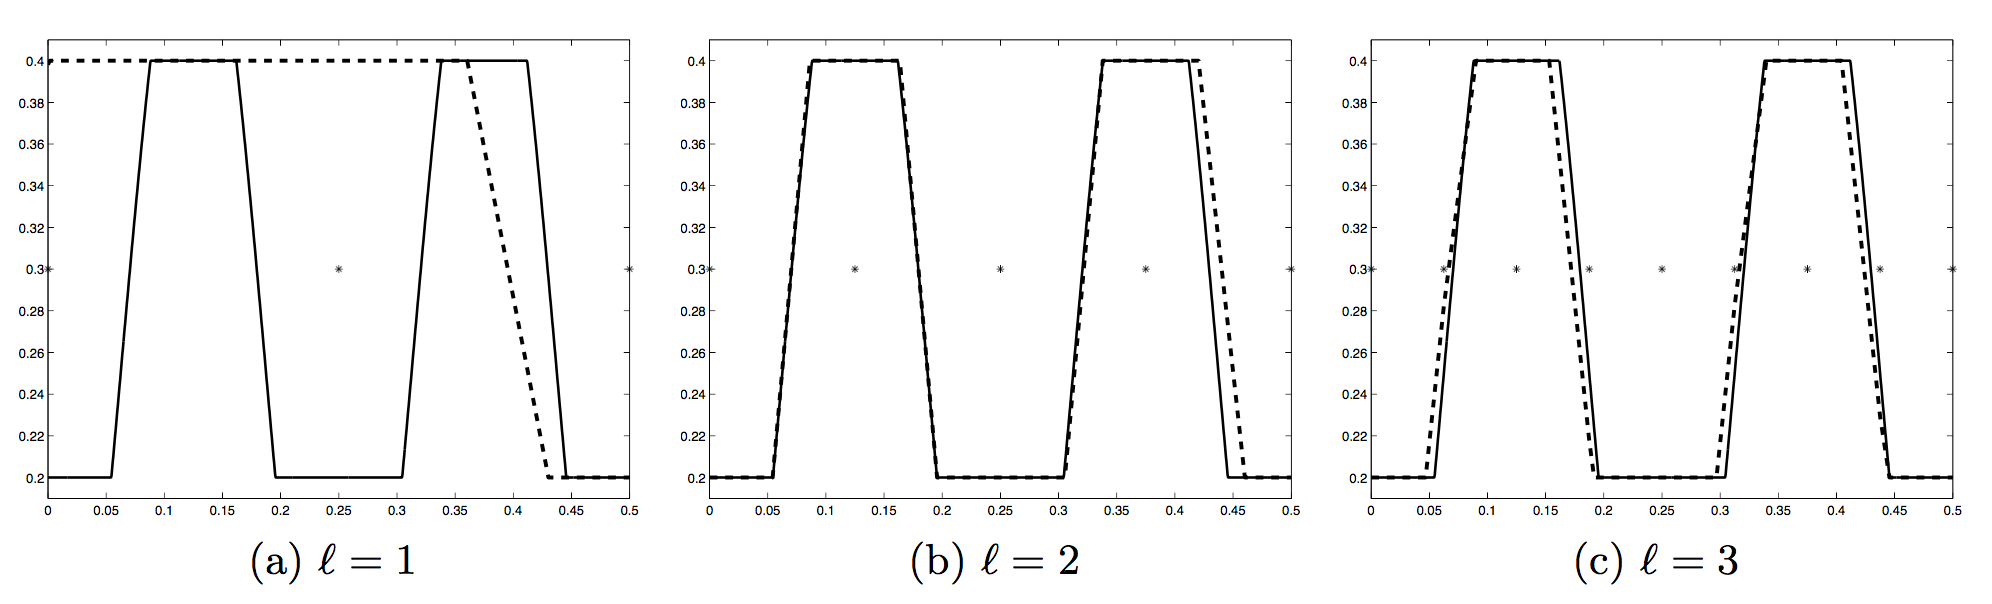
\includegraphics[width=\linewidth]{img/cap6/TestCase02_ues_paper}
\caption{Test Case 02 $\overline{u}$ e $u_k$ risultati di \cite{MAIN}}
\label{fig:503}
\end{figure}

\begin{figure}
\centering%
\subfigure[\protect\url{l = 1}]%
{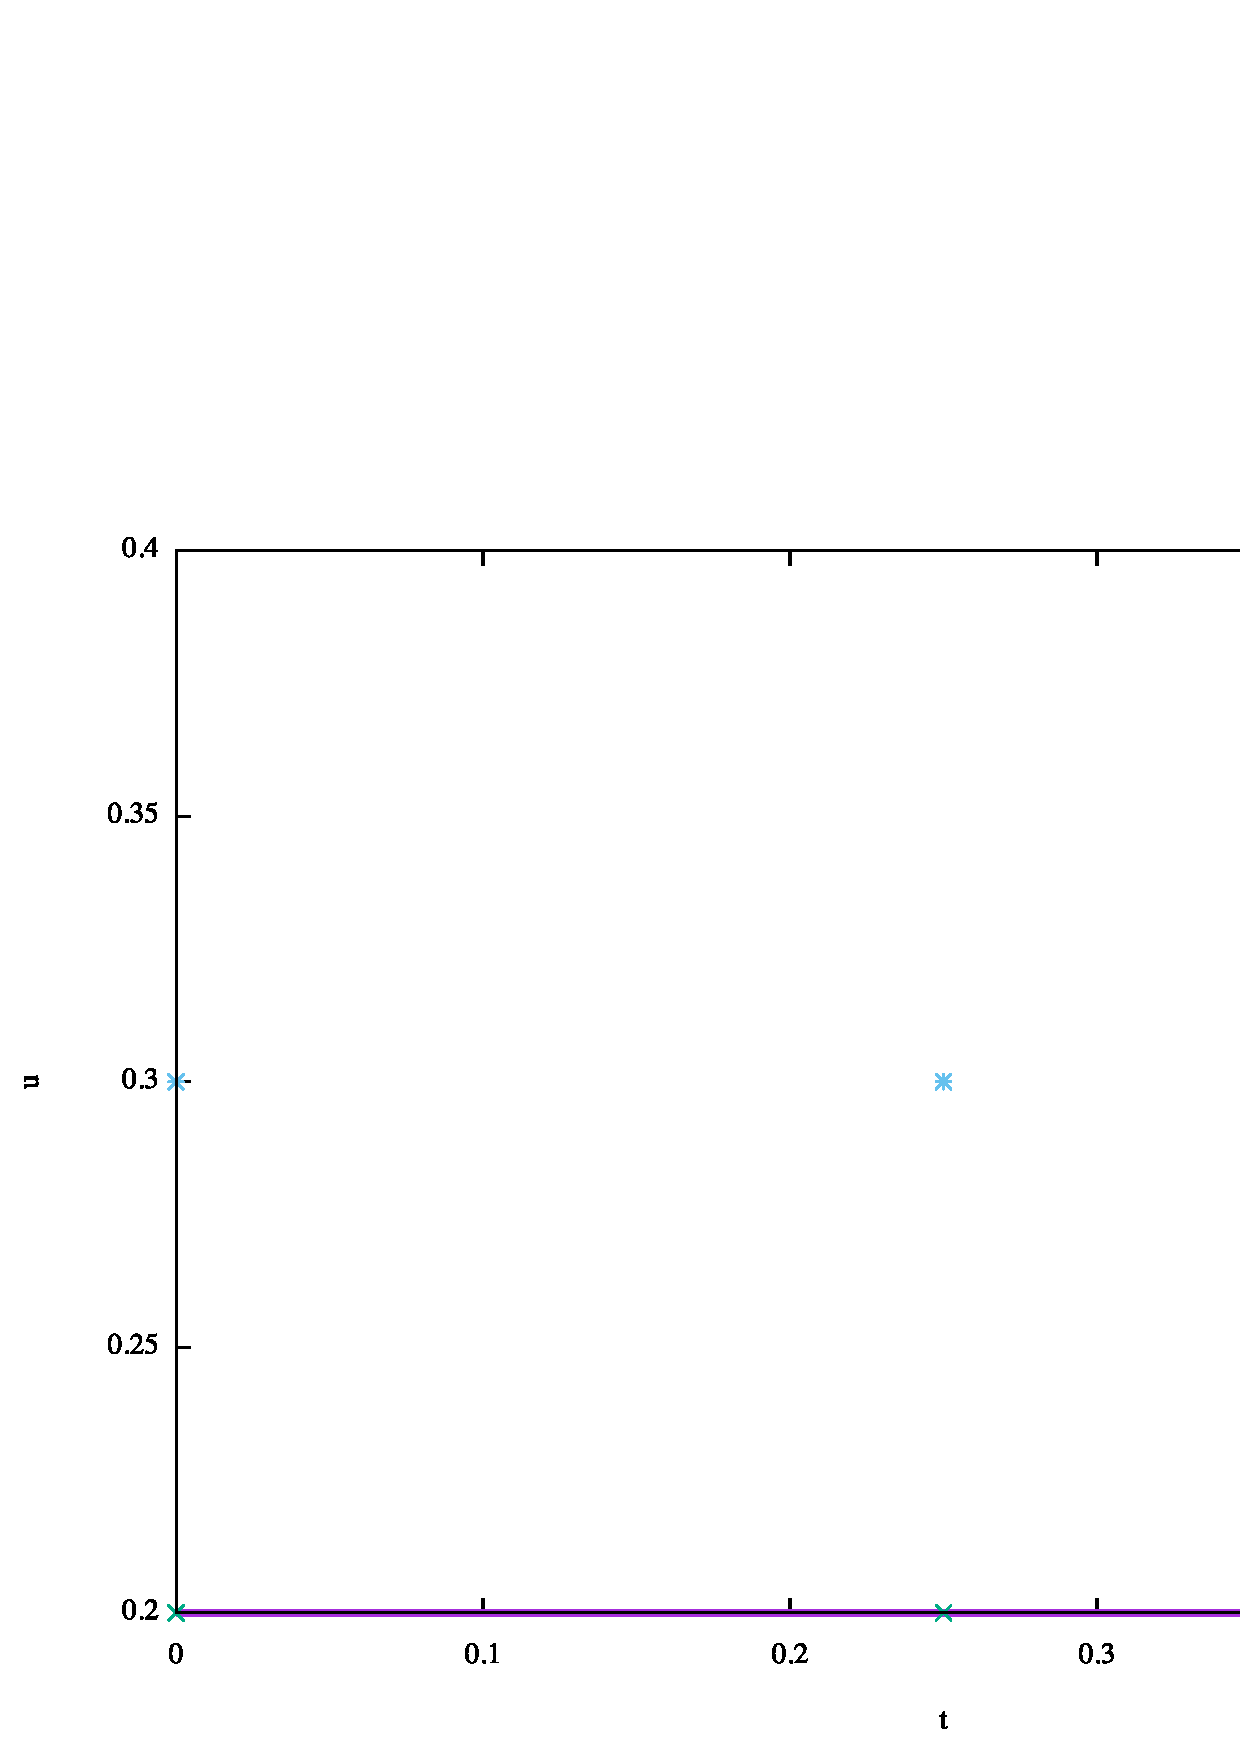
\includegraphics[width=0.3\linewidth]{img/cap6/Imm_PF_02/ControlSol_N150_l1}}\qquad
\subfigure[\protect\url{l = 2}]%
{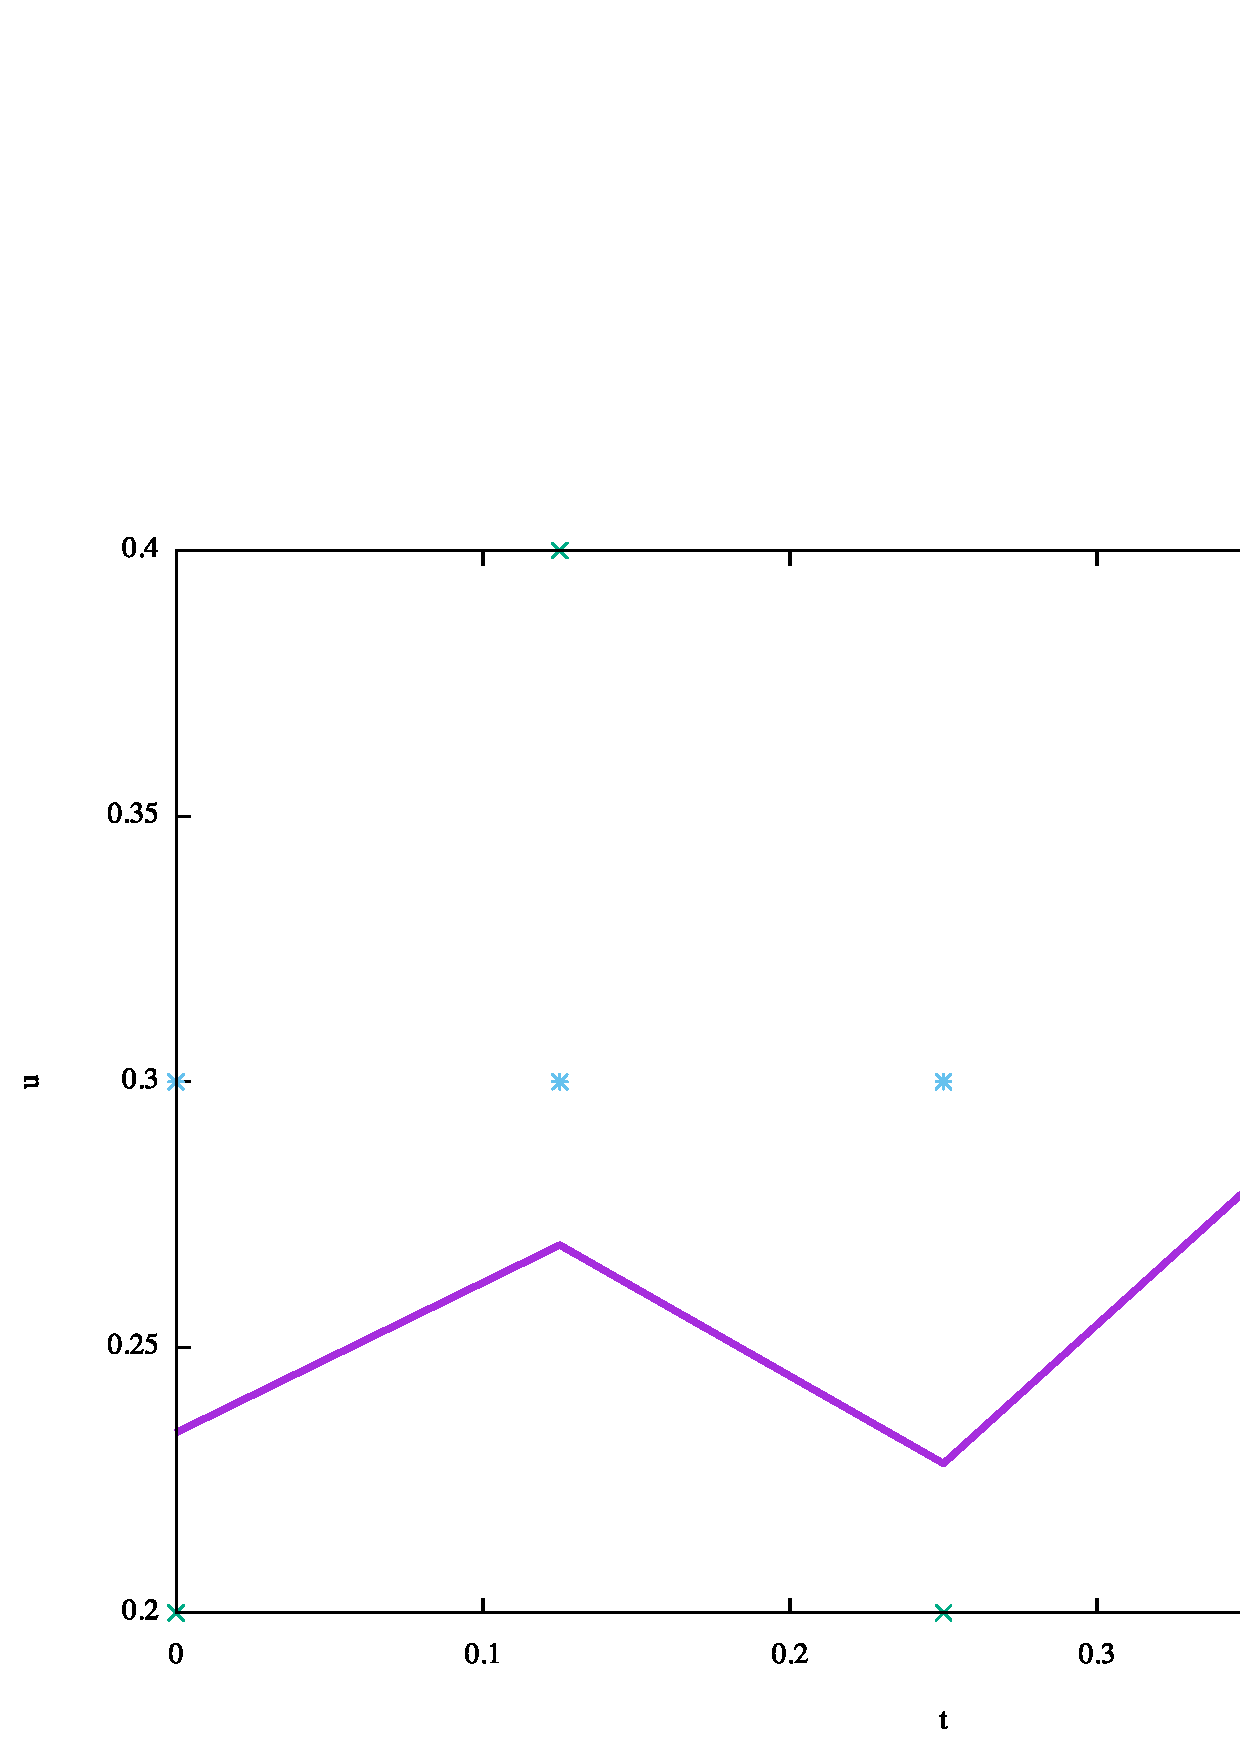
\includegraphics[width=0.3\linewidth]{img/cap6/Imm_PF_02/ControlSol_N150_l2}}\qquad
\subfigure[\protect\url{l = 3}]%
{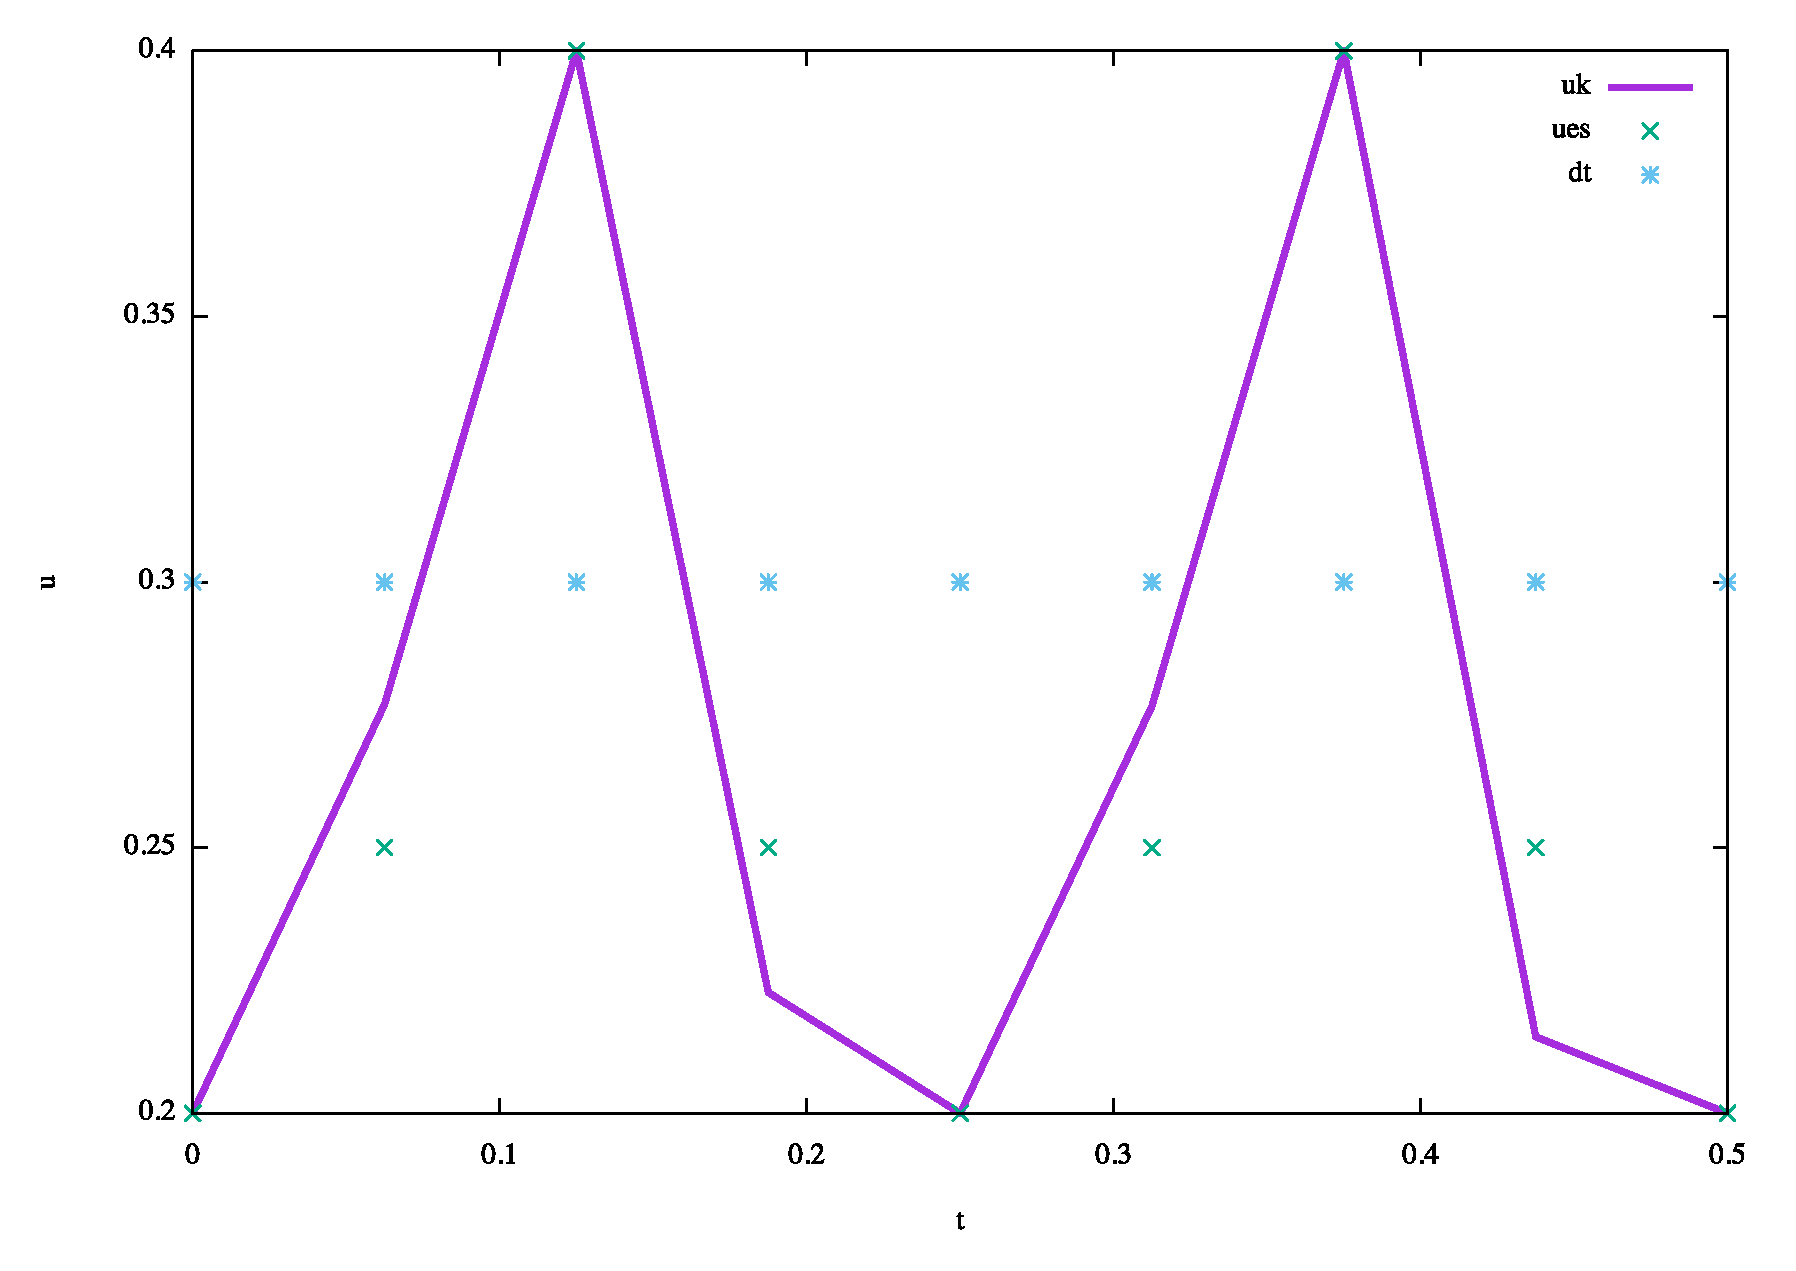
\includegraphics[width=0.3\linewidth]{img/cap6/Imm_PF_02/ControlSol_N150_l3}}\qquad
\subfigure[\protect\url{l = 4}]%
{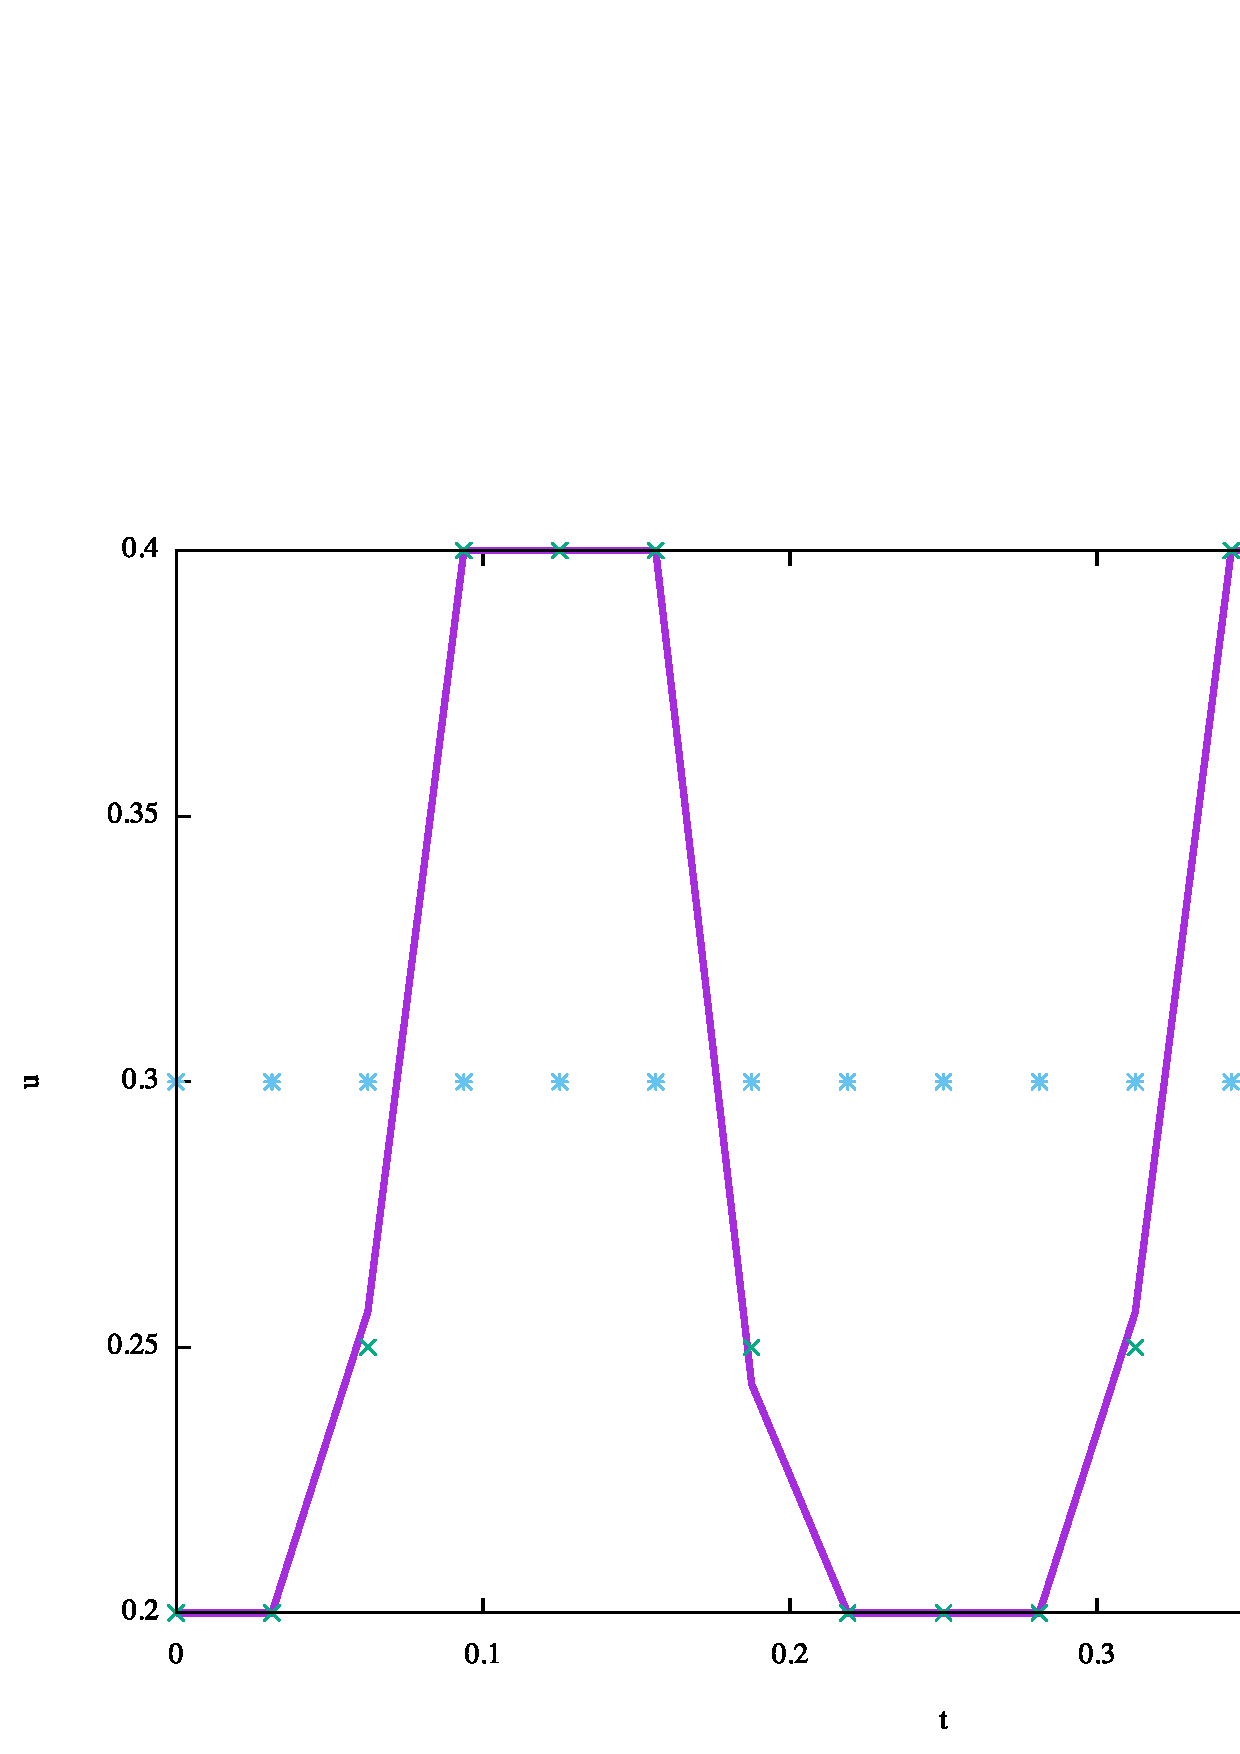
\includegraphics[width=0.3\linewidth]{img/cap6/Imm_PF_02/ControlSol_N150_l4}}\qquad
\subfigure[\protect\url{l = 5}]%
{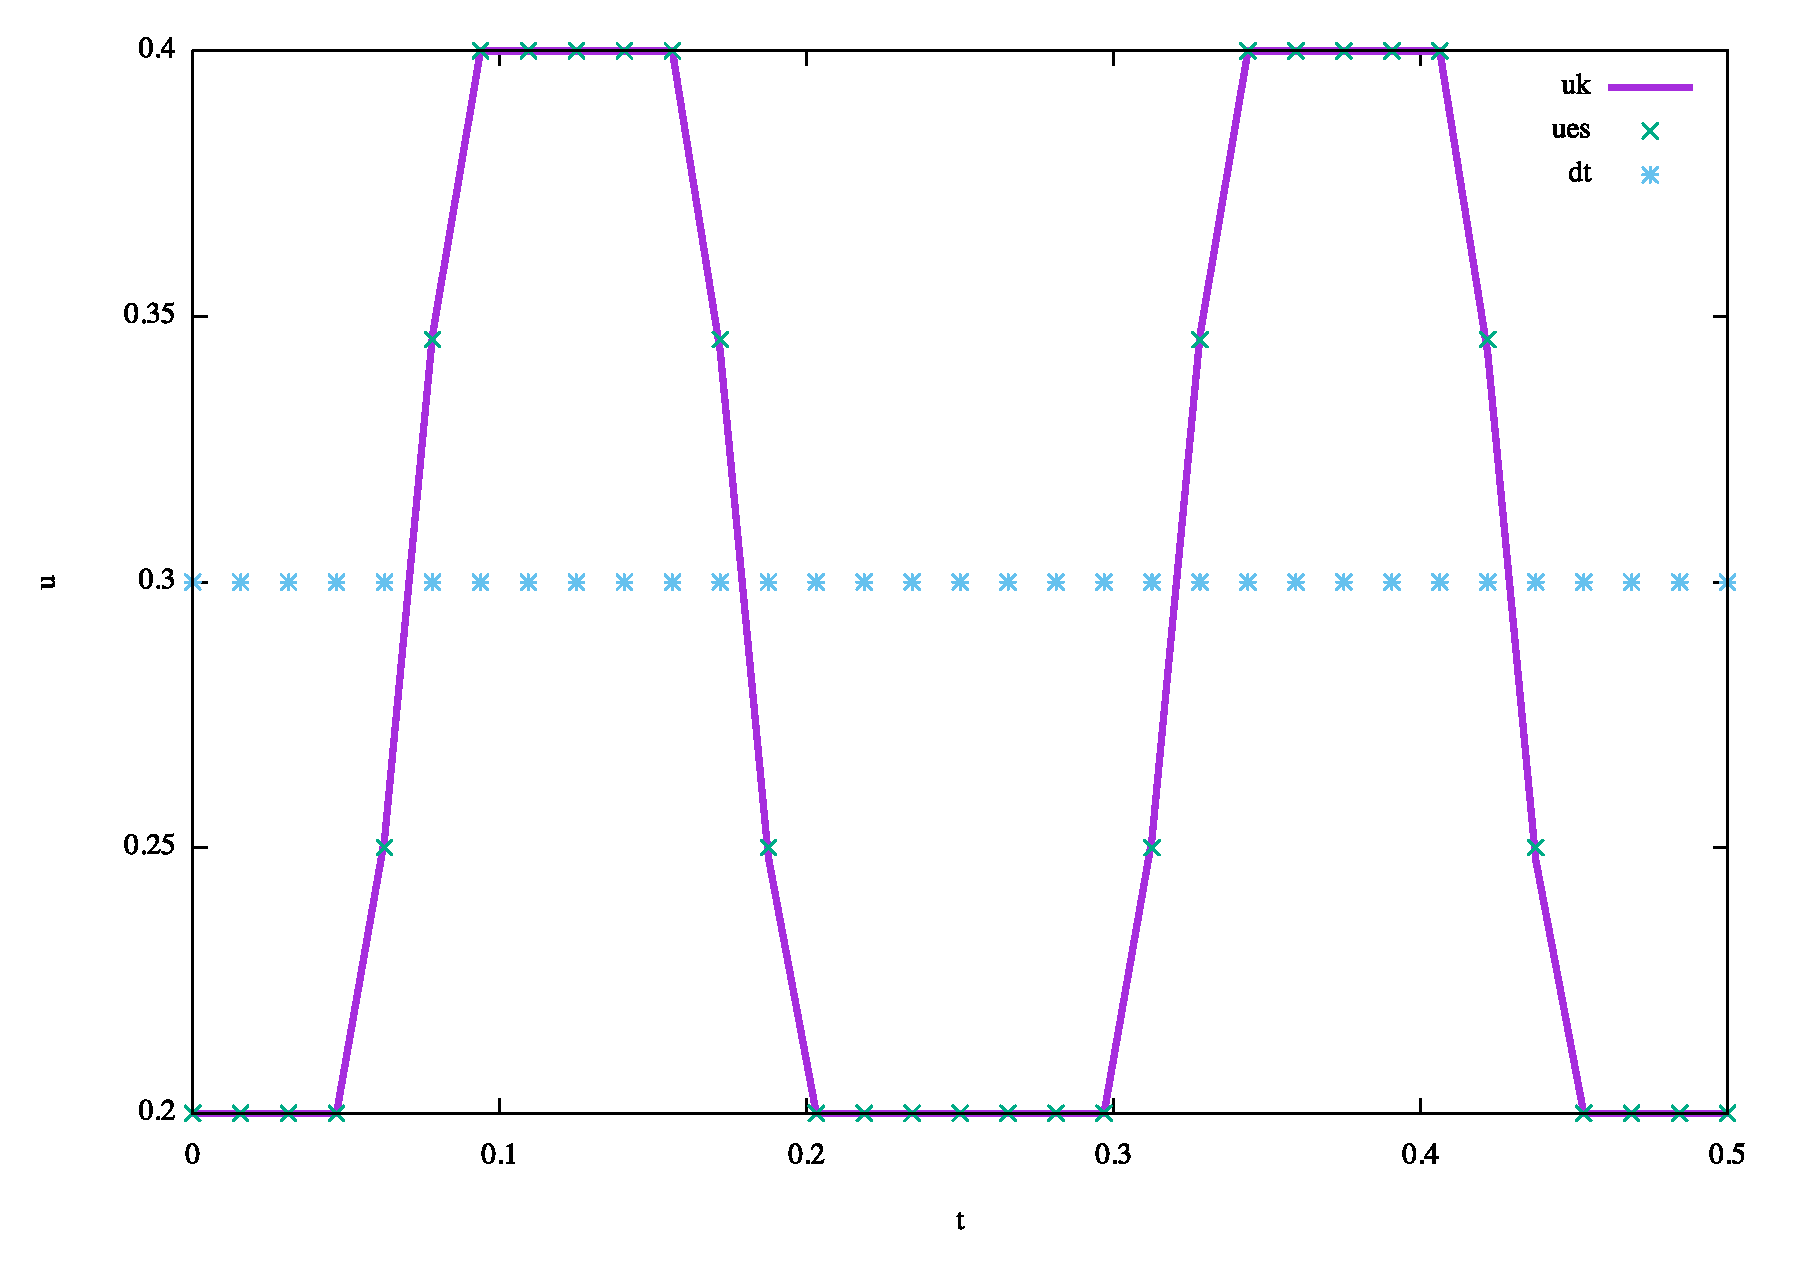
\includegraphics[width=0.3\linewidth]{img/cap6/Imm_PF_02/ControlSol_N150_l5}}\qquad
\subfigure[\protect\url{l = 6}]%
{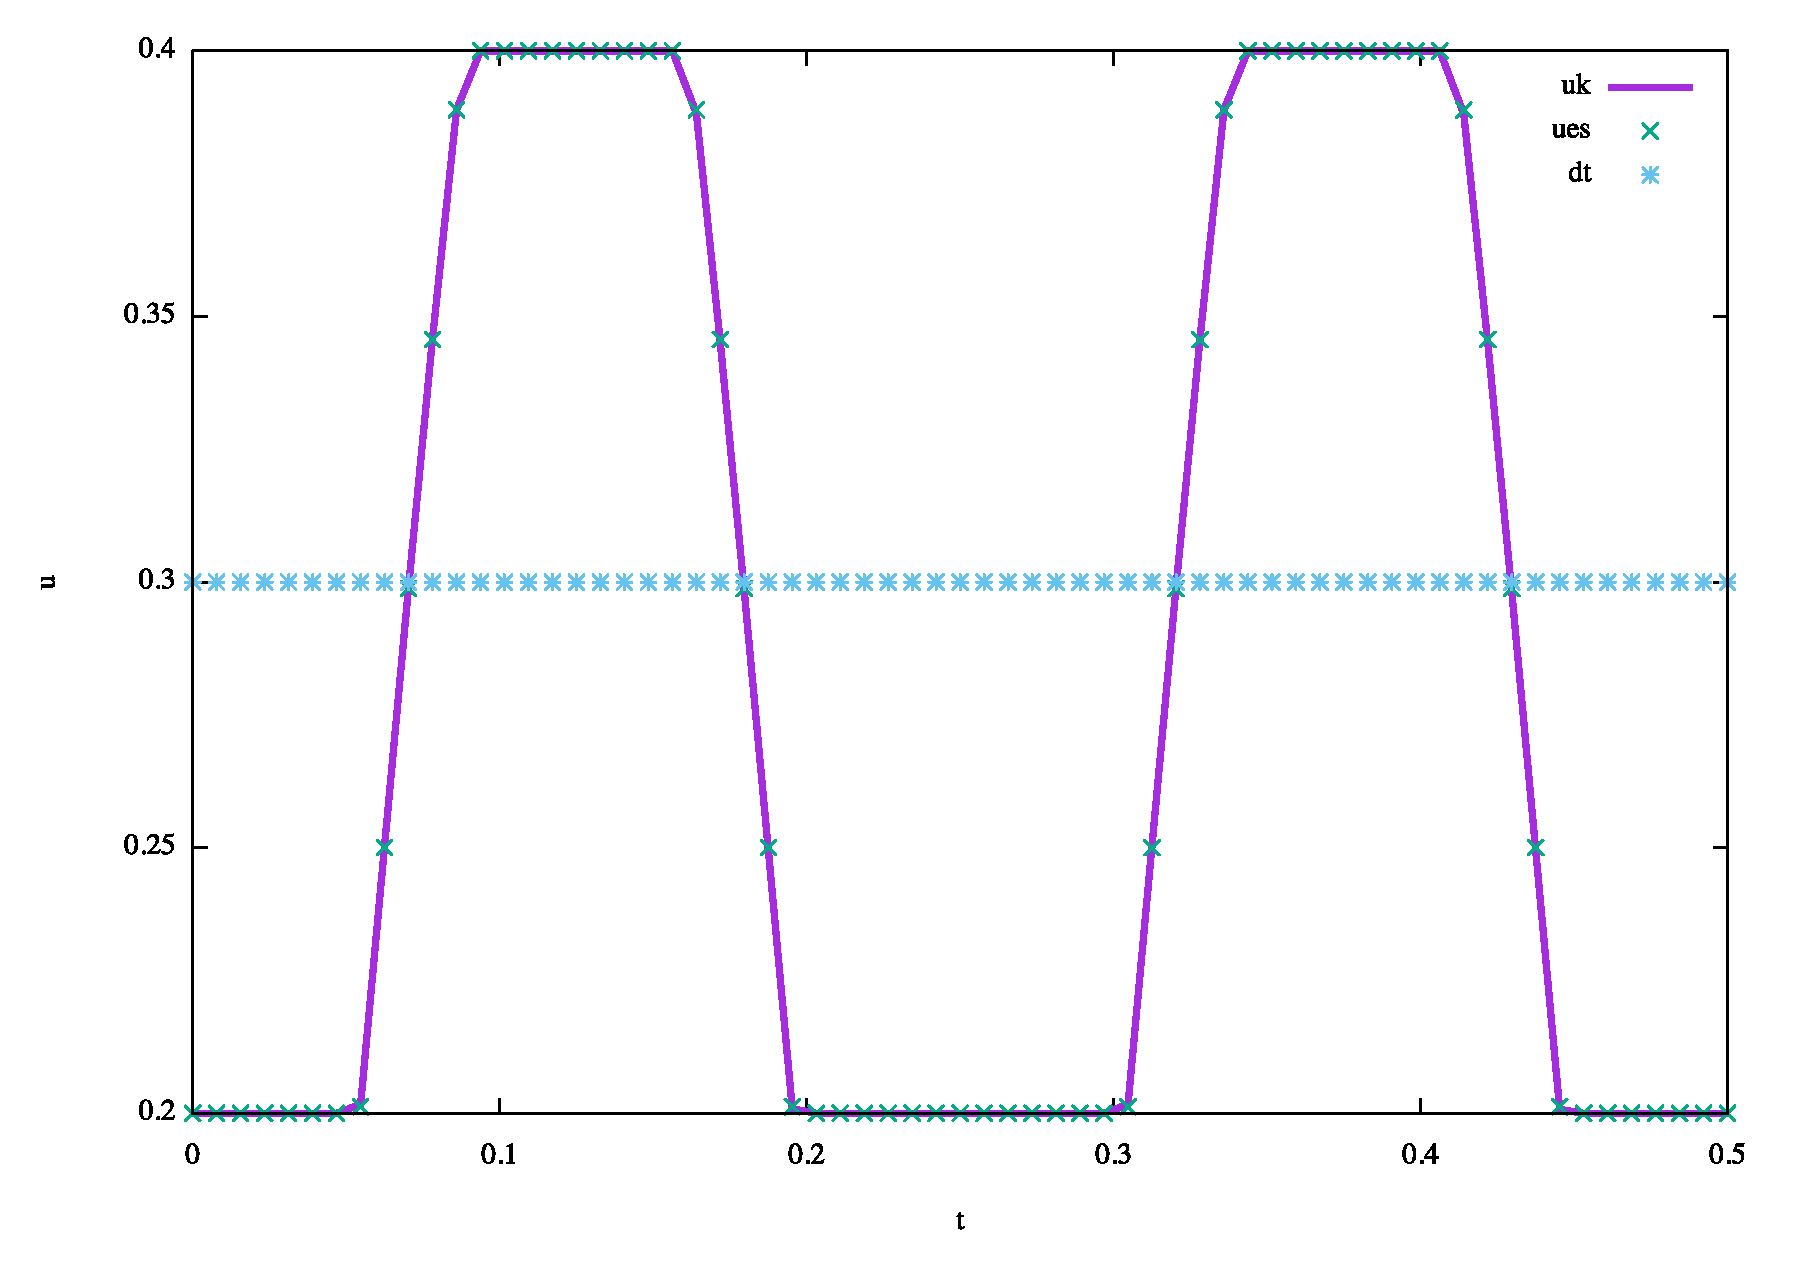
\includegraphics[width=0.3\linewidth]{img/cap6/Imm_PF_02/ControlSol_N150_l6}}\qquad
\subfigure[\protect\url{l = 7}]%
{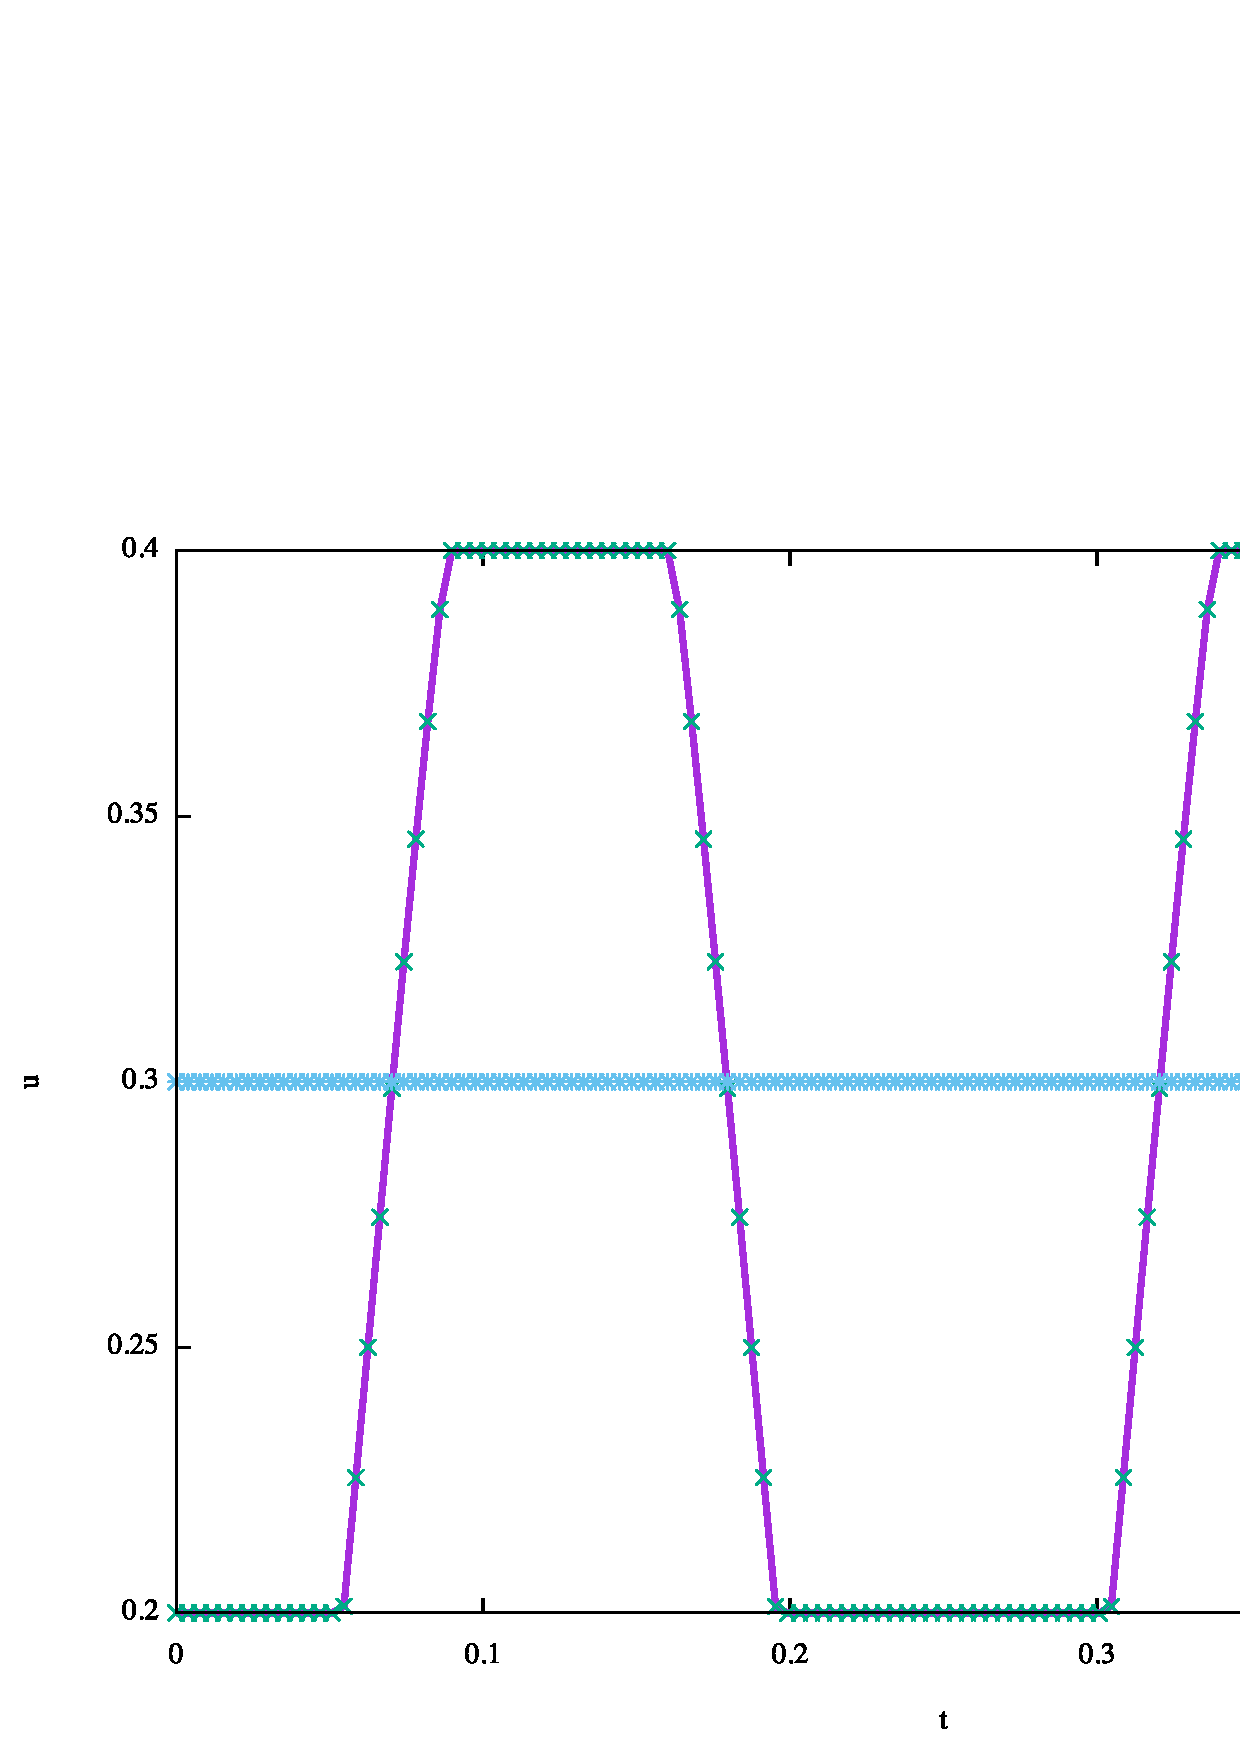
\includegraphics[width=0.3\linewidth]{img/cap6/Imm_PF_02/ControlSol_N150_l7}}\qquad
\subfigure[\protect\url{l = 8}]%
{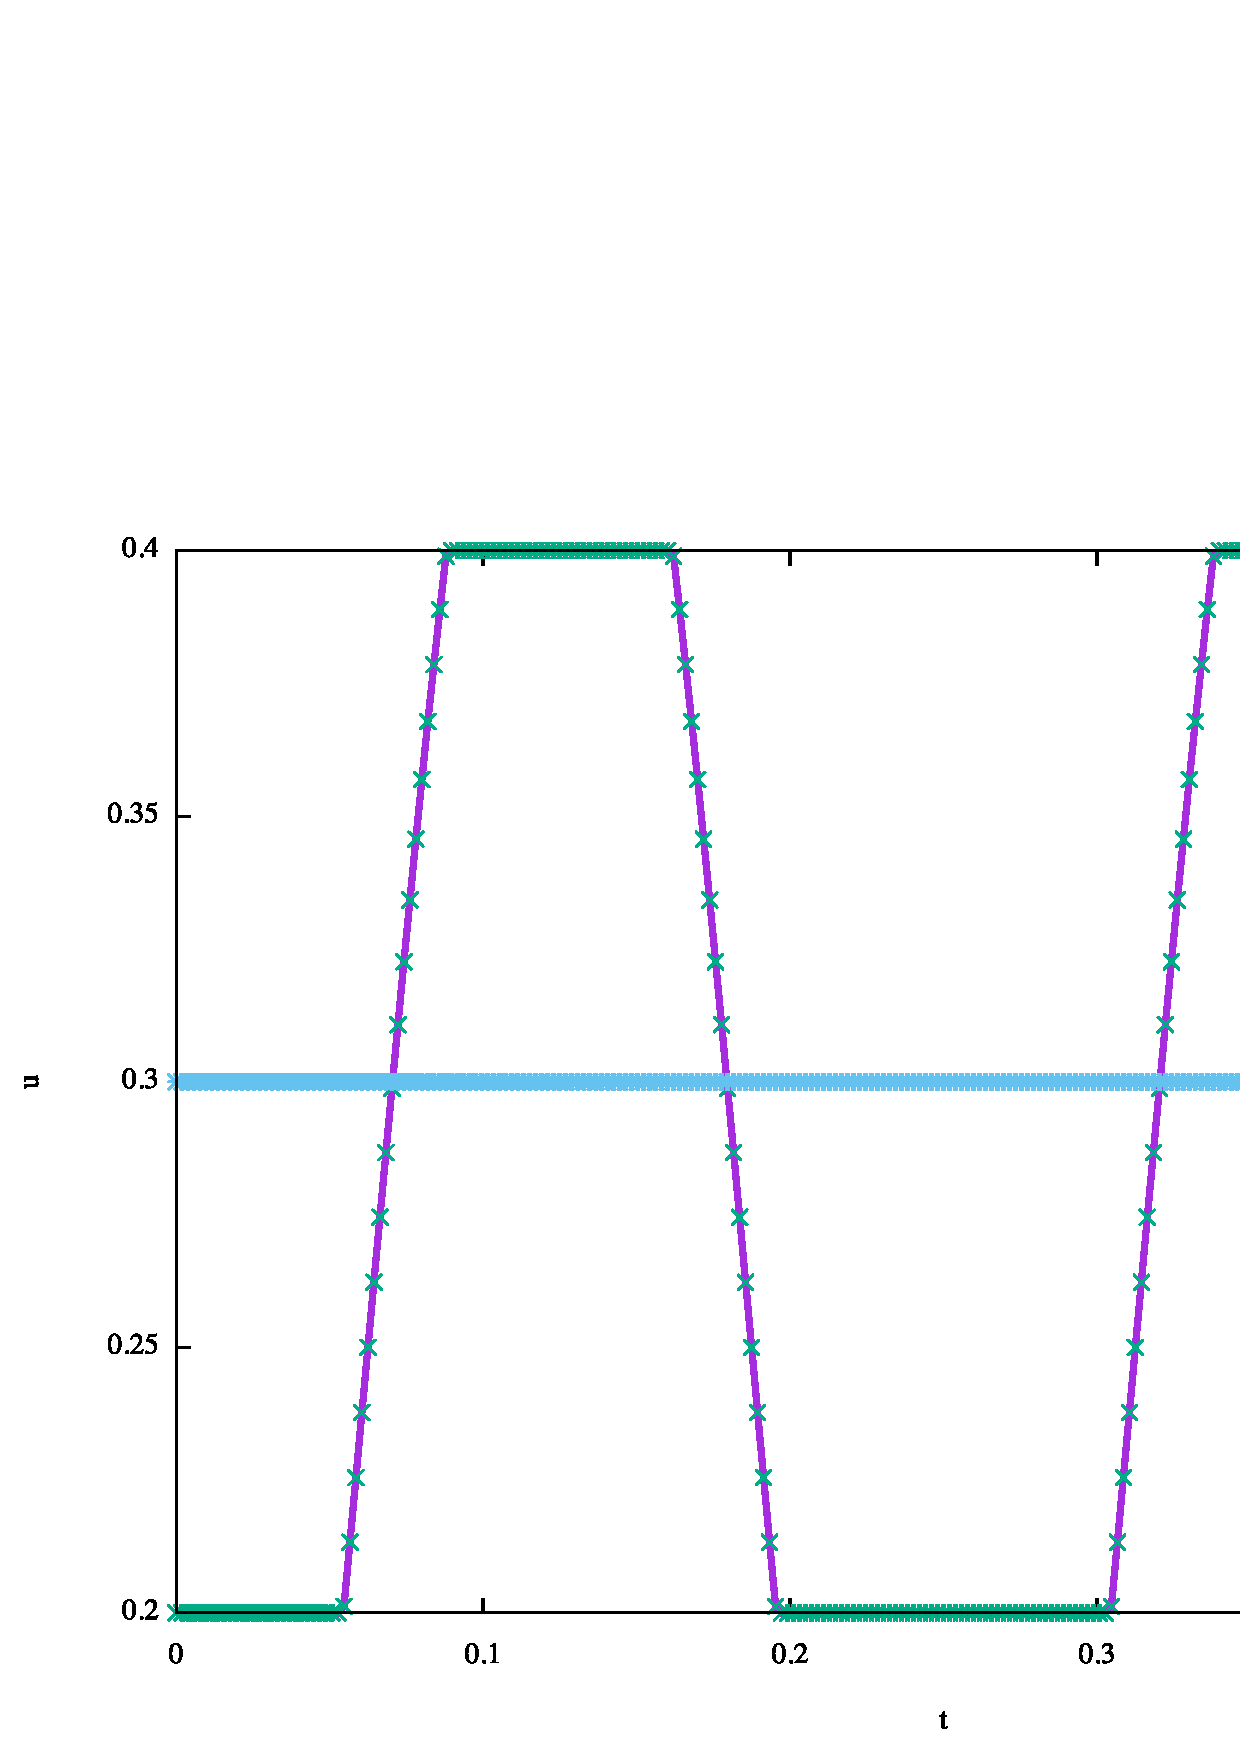
\includegraphics[width=0.3\linewidth]{img/cap6/Imm_PF_02/ControlSol_N150_l8}}
\caption{Test Case 02 $\overline{u}$ e $u_k$ risultati dell'algoritmo di punto fisso}
\label{fig:504}
\end{figure}

\begin{figure}
\centering%
\subfigure[\protect\url{l = 1}]%
{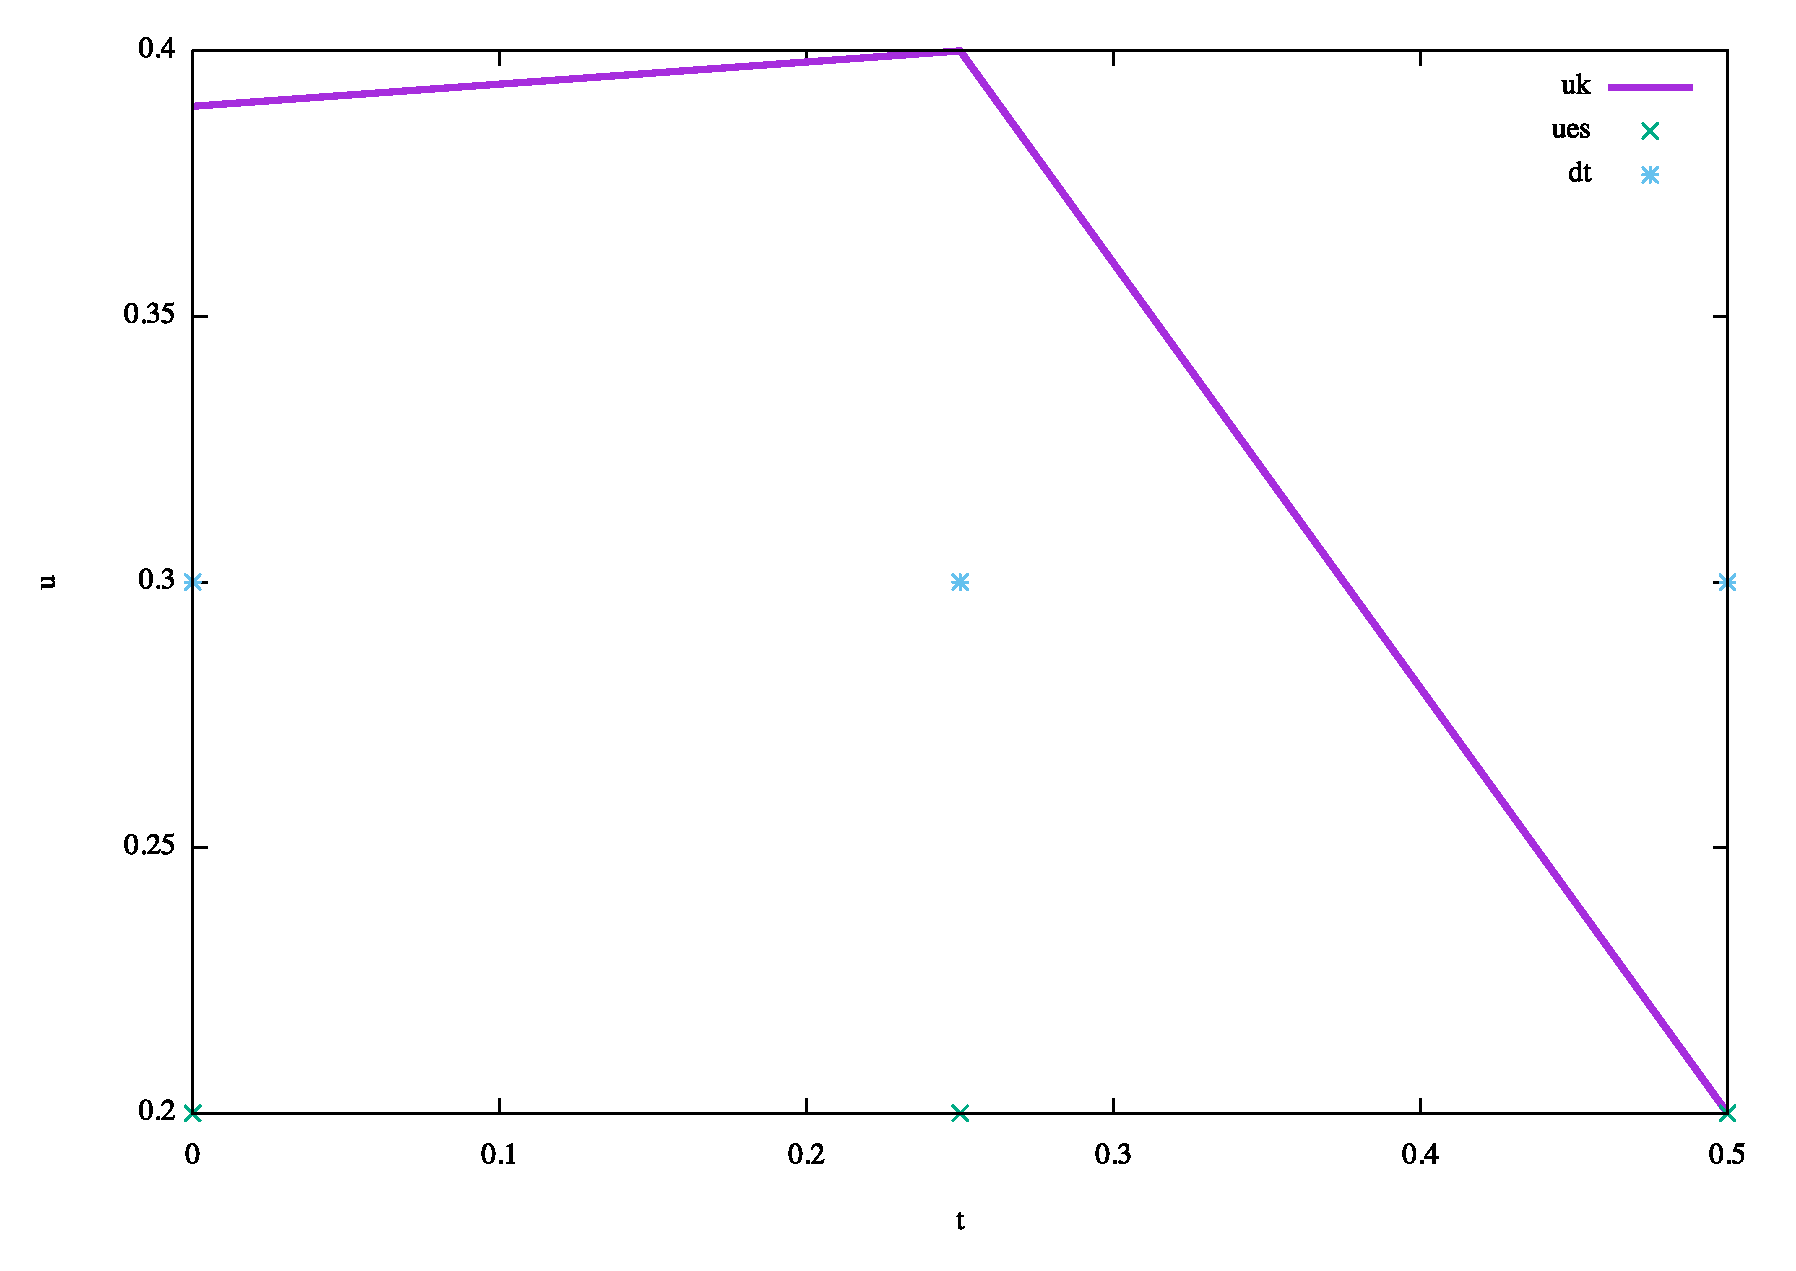
\includegraphics[width=0.3\linewidth]{img/cap6/Imm_CG_02/ControlSol_N150_l1}}\qquad
\subfigure[\protect\url{l = 2}]%
{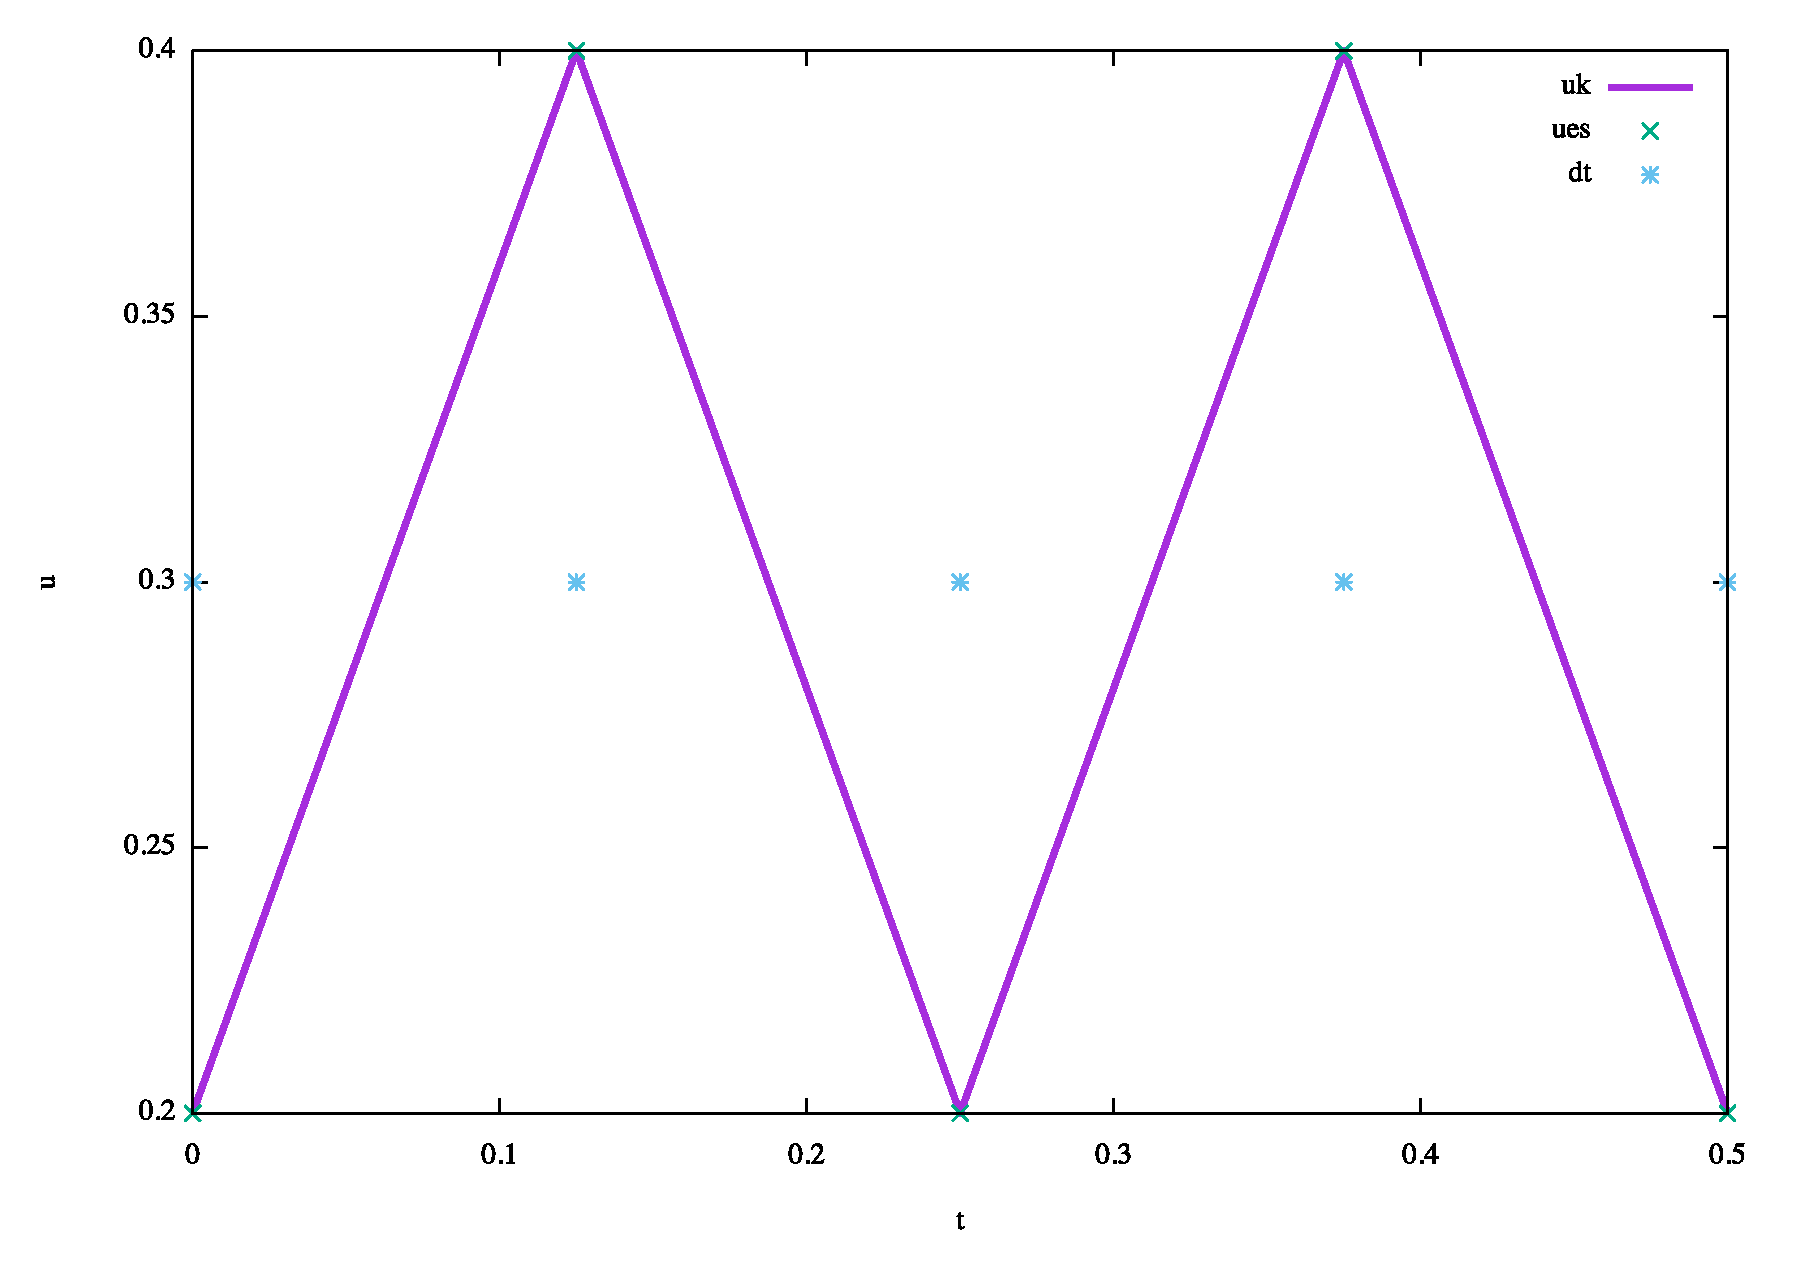
\includegraphics[width=0.3\linewidth]{img/cap6/Imm_CG_02/ControlSol_N150_l2}}\qquad
\subfigure[\protect\url{l = 3}]%
{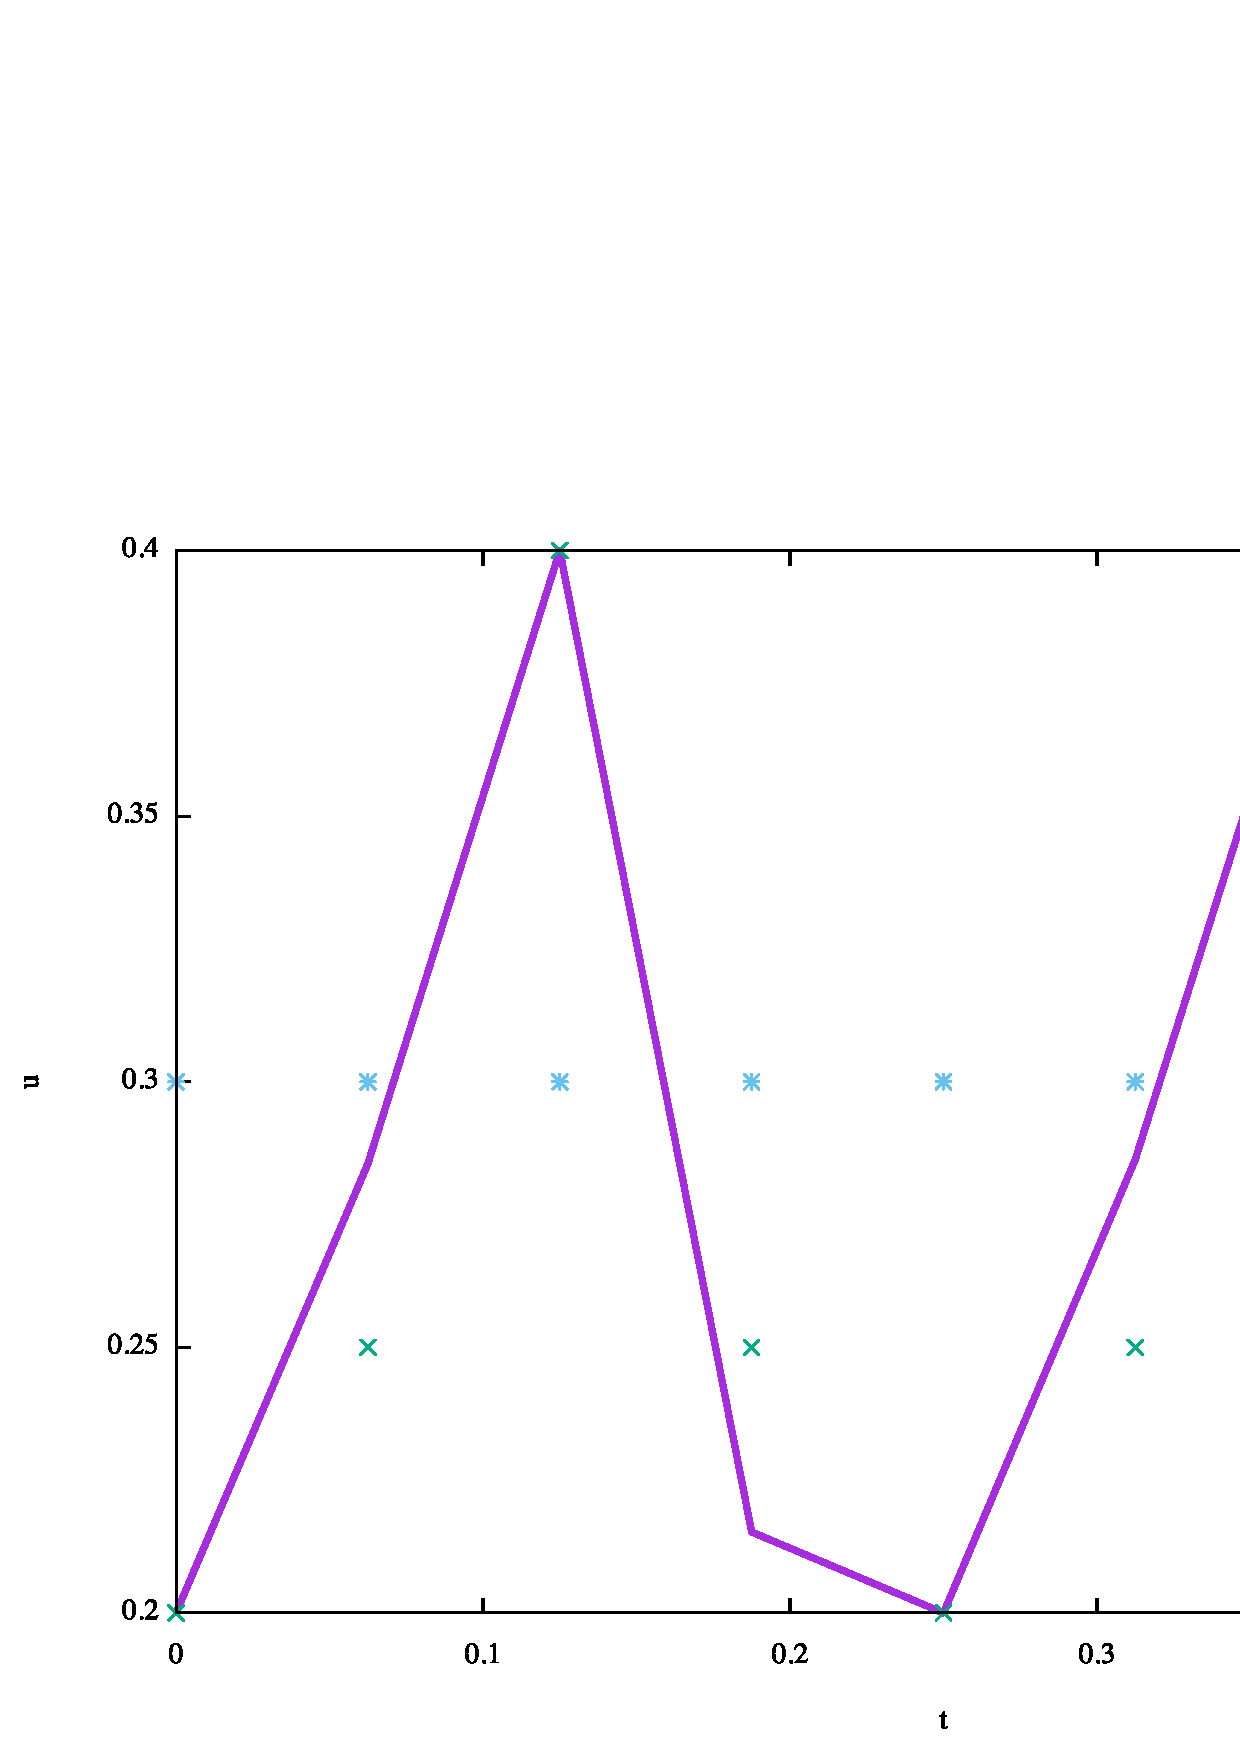
\includegraphics[width=0.3\linewidth]{img/cap6/Imm_CG_02/ControlSol_N150_l3}}\qquad
\subfigure[\protect\url{l = 4}]%
{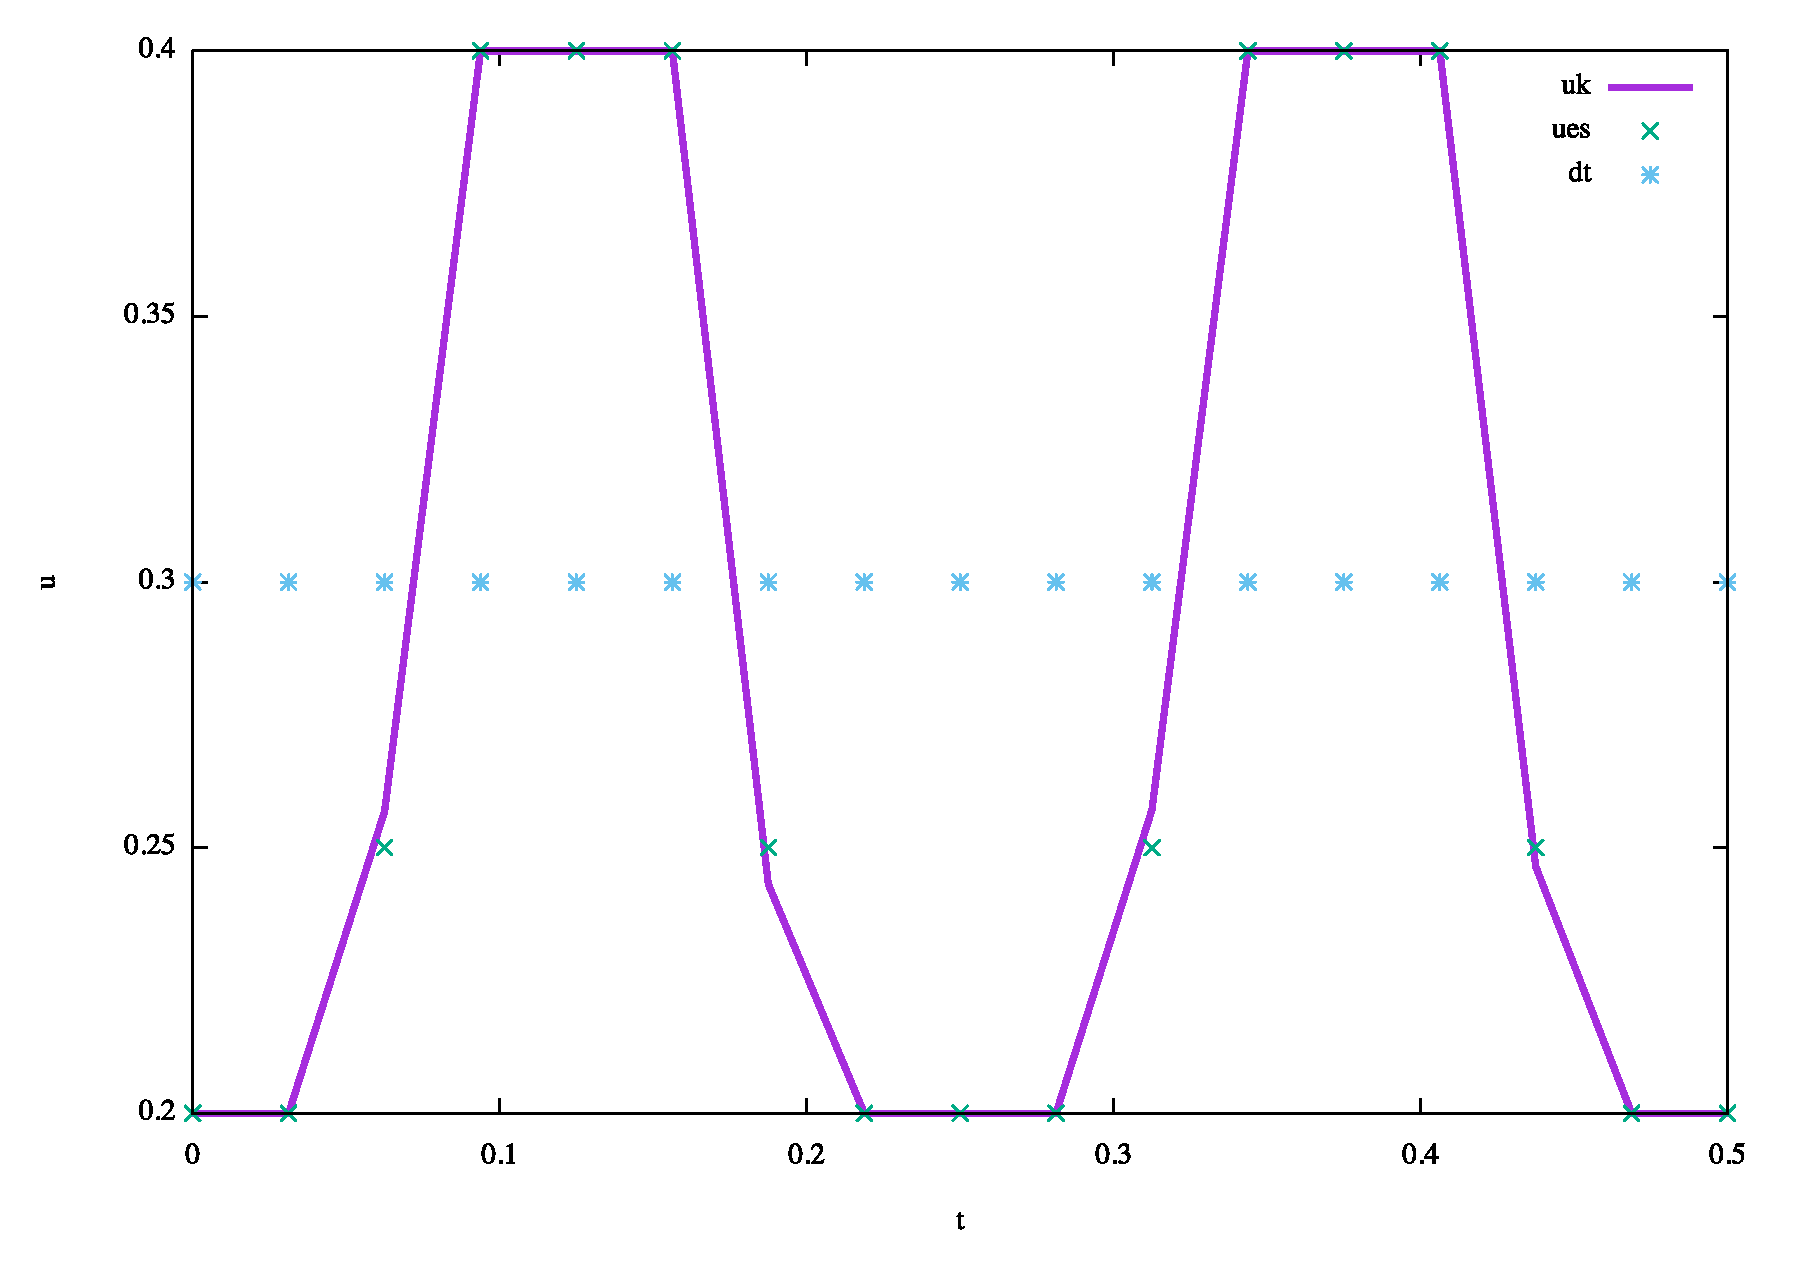
\includegraphics[width=0.3\linewidth]{img/cap6/Imm_CG_02/ControlSol_N150_l4}}\qquad
\subfigure[\protect\url{l = 5}]%
{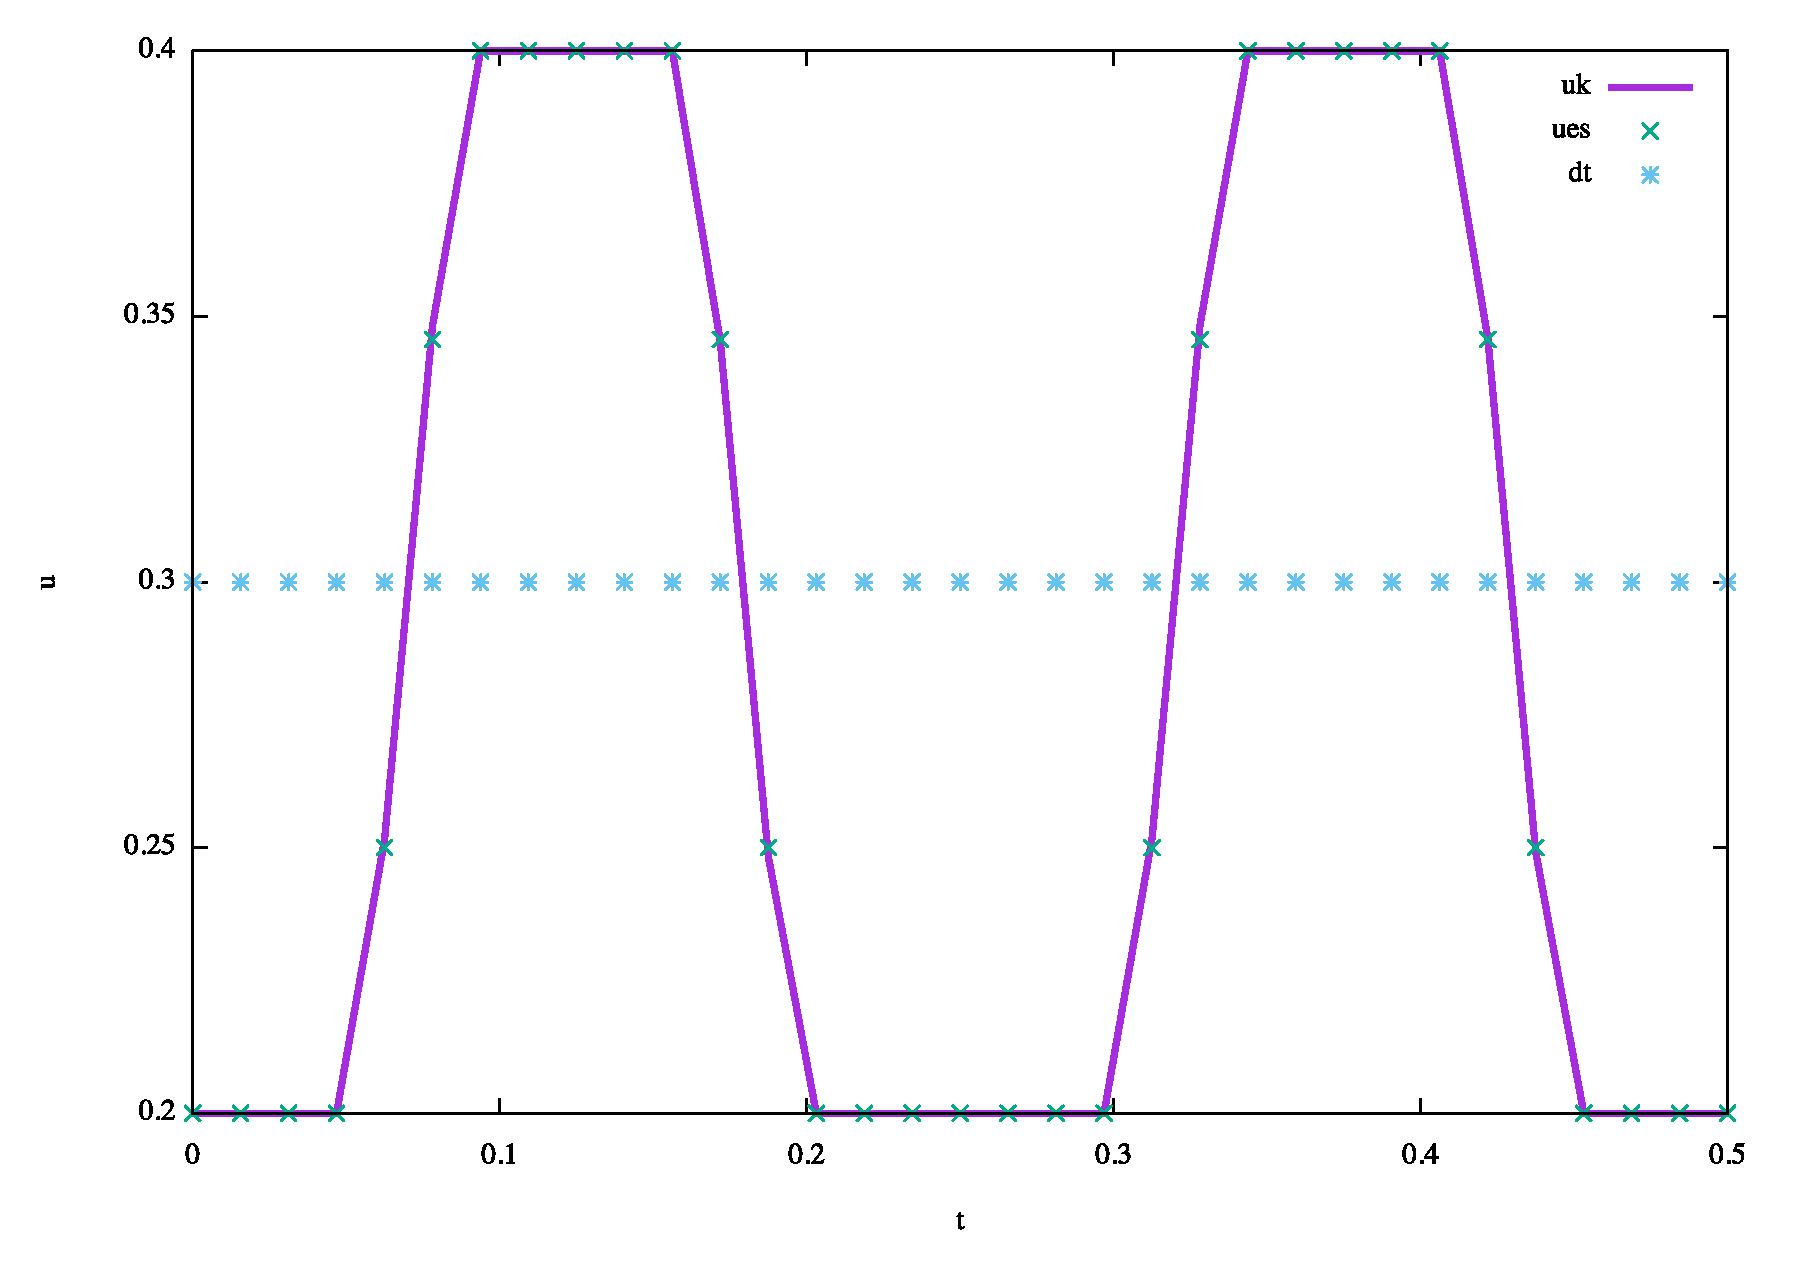
\includegraphics[width=0.3\linewidth]{img/cap6/Imm_CG_02/ControlSol_N150_l5}}\qquad
\subfigure[\protect\url{l = 6}]%
{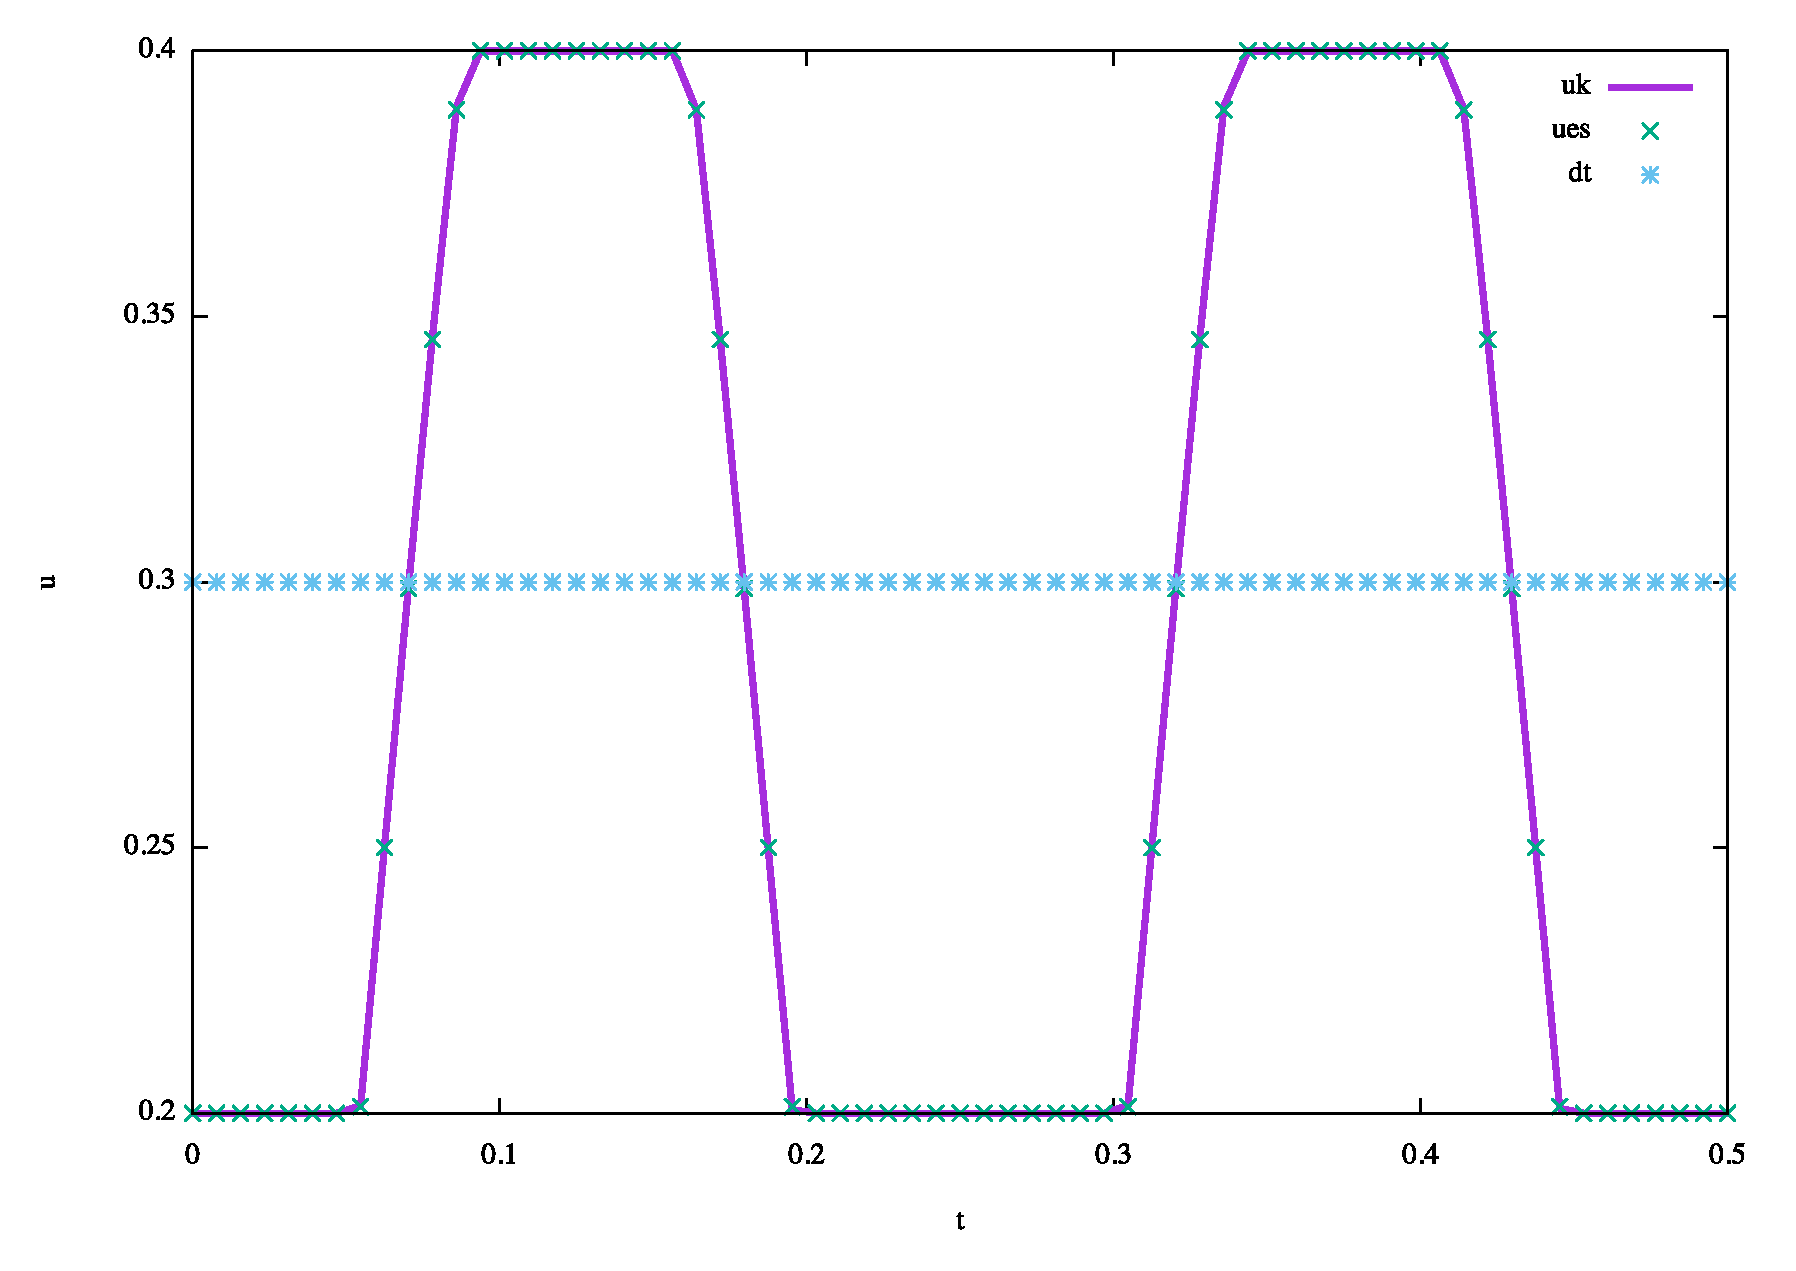
\includegraphics[width=0.3\linewidth]{img/cap6/Imm_CG_02/ControlSol_N150_l6}}\qquad
\subfigure[\protect\url{l = 7}]%
{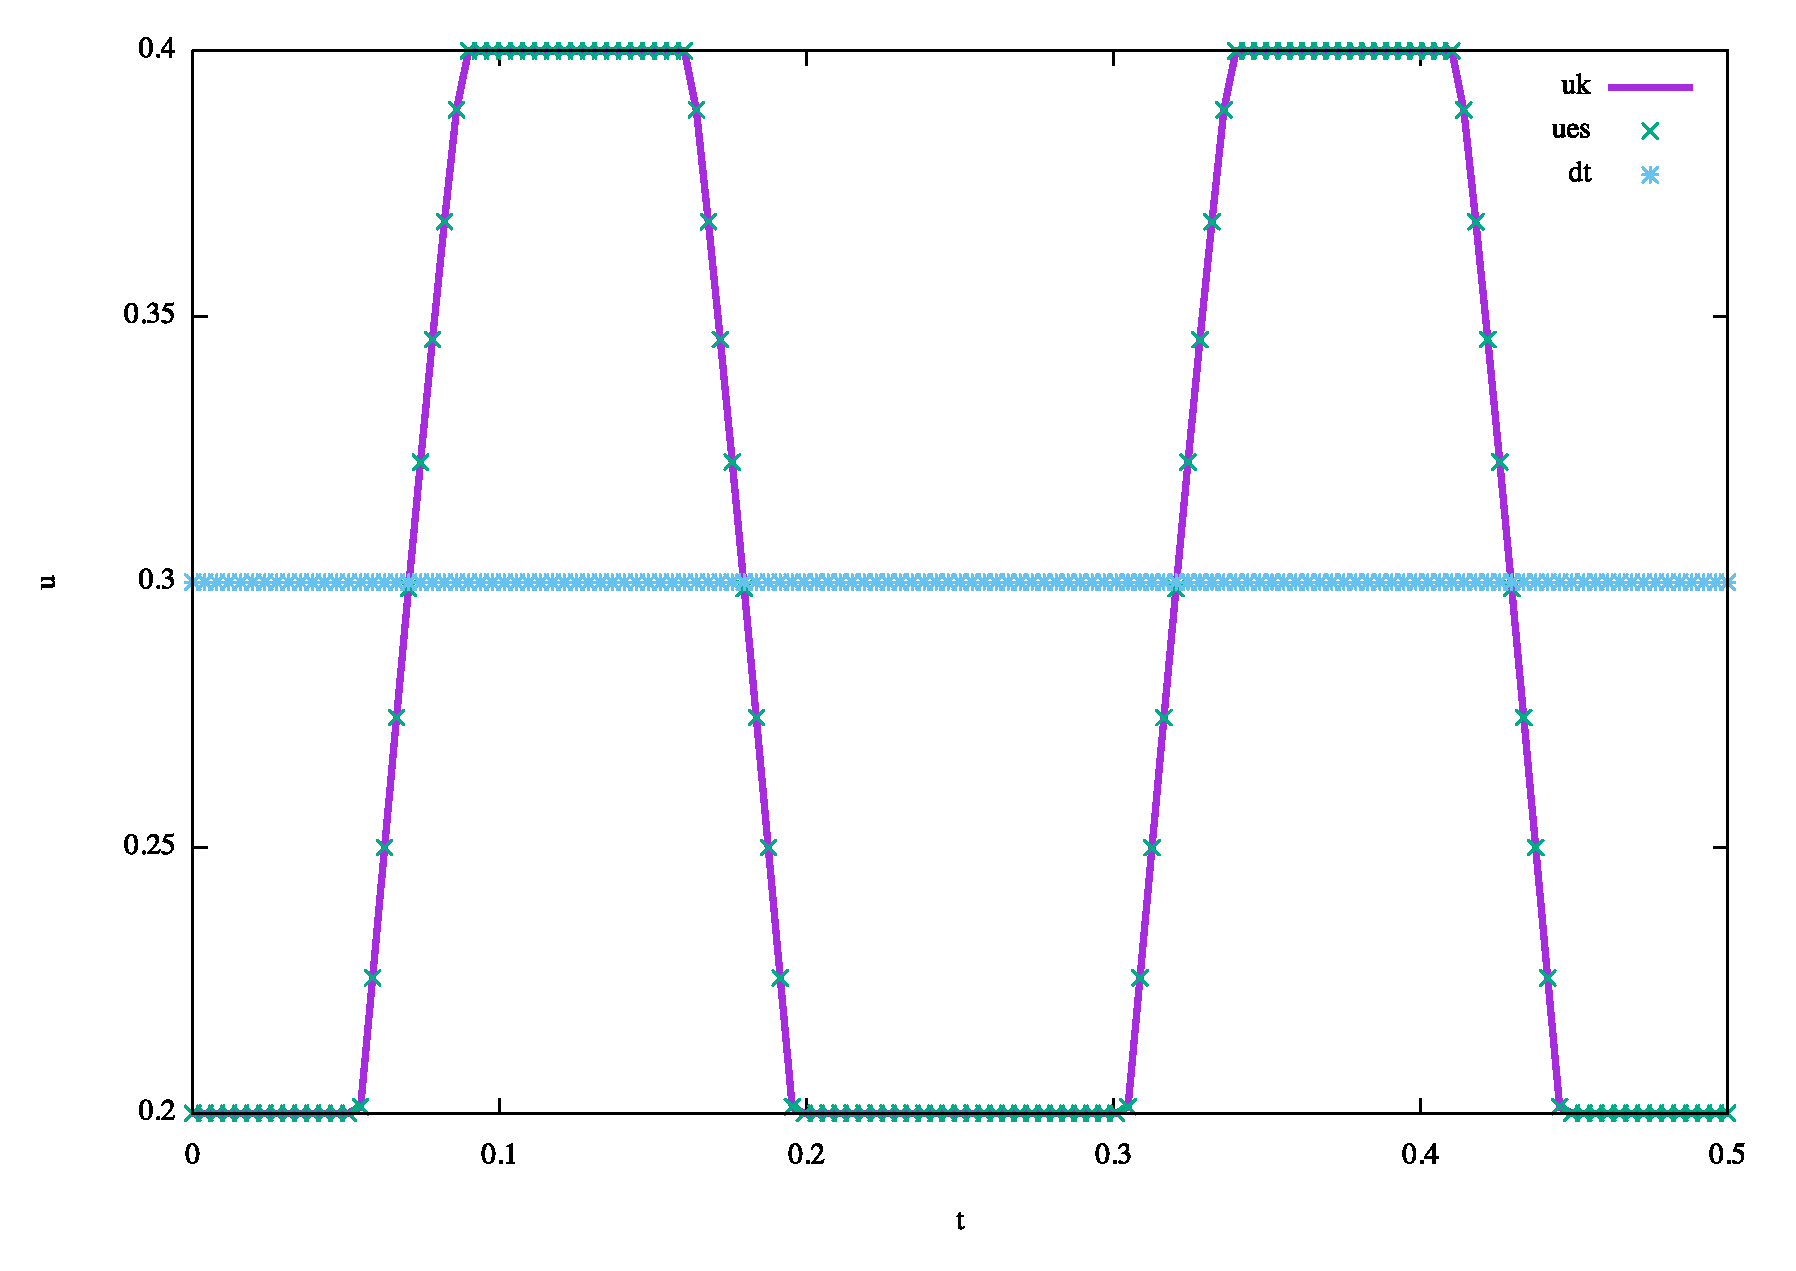
\includegraphics[width=0.3\linewidth]{img/cap6/Imm_CG_02/ControlSol_N150_l7}}\qquad
\subfigure[\protect\url{l = 8}]%
{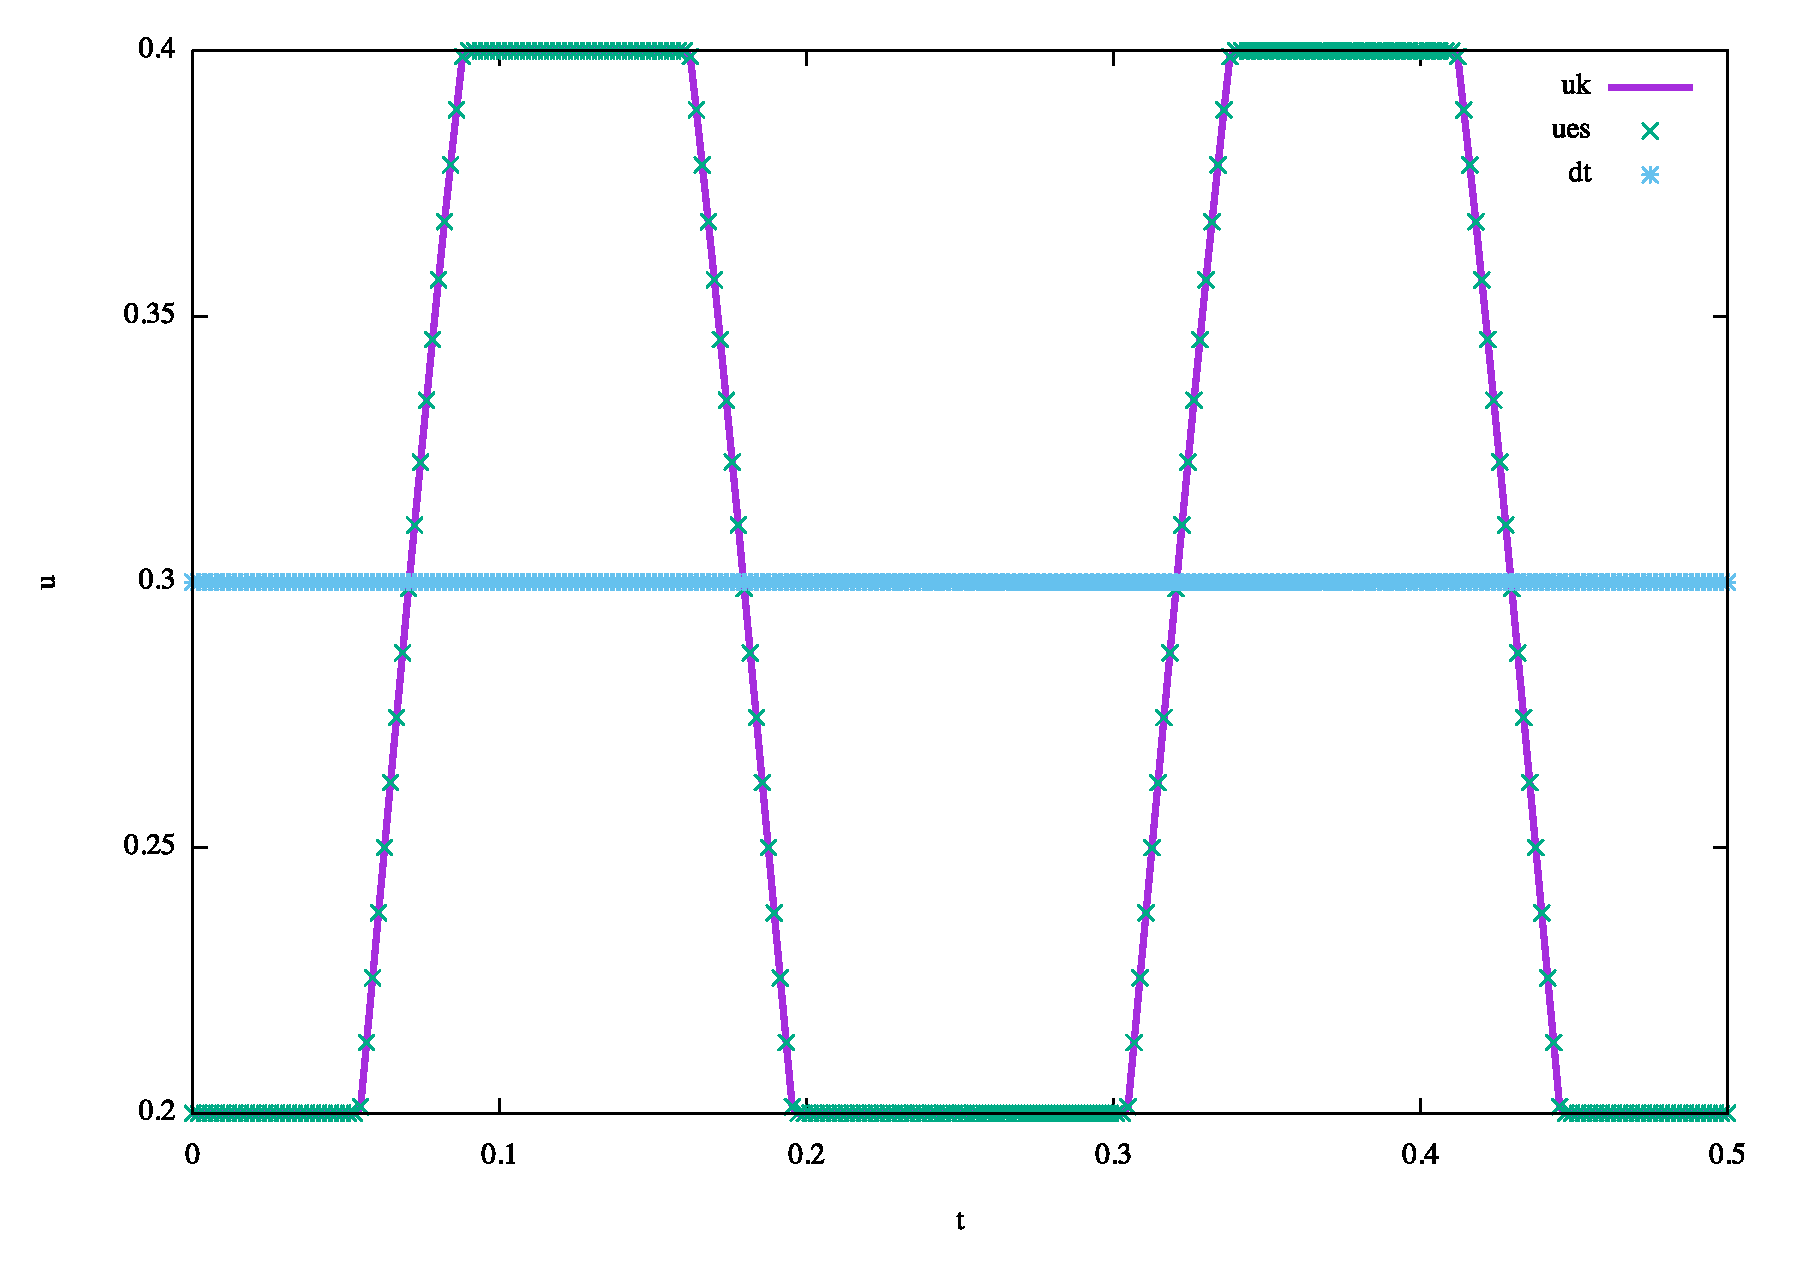
\includegraphics[width=0.3\linewidth]{img/cap6/Imm_CG_02/ControlSol_N150_l8}}
\caption{Test Case 02 $\overline{u}$ e $u_k$: risultati dell'algortimod di semi newton}
\label{fig:505}
\end{figure}